\documentclass[conference]{IEEEtran}
% Final (Phase II) report. Every section is its own file in sections/ so that
% each member edits and commits only the files they own (docs/phase2_work_split.md).
% Tables and plots read the numbers generated by tools/sweep.py (data/*.dat) and
% tools/area_table.py (data/area.tex); do not type results by hand.
% The Phase I report is kept unchanged in phase1/.
\usepackage[T1]{fontenc}
\usepackage{mathptmx}
\usepackage{amsmath}
\usepackage{booktabs}
\usepackage{graphicx}
\usepackage{array}
\usepackage{url}
\usepackage{tikz}
\usetikzlibrary{arrows.meta,positioning,calc,fit}
\usepackage{pgfplots}
\pgfplotsset{compat=1.18}
\usepackage[hidelinks]{hyperref}

\newcommand{\sig}[1]{\texttt{#1}}
% table bodies generated by the scripts: the TeX primitive \@@input is expandable,
% so \bottomrule after it is still at the start of a row
\makeatletter
\newcommand{\tabinput}[1]{\@@input #1 }
\makeatother

\begin{document}

\title{Instruction and Data Memory Hierarchy:\\
From a Harvard Organisation to Split Caches\\over a Shared Memory}

\author{\IEEEauthorblockN{Yashpal, Anshika, Ankit, Samriddhi, Ayush}
\IEEEauthorblockA{Modern Computer Architecture, Project 9 (Final Report, Phases I and II)\\
Department of Computer Science and Artificial Intelligence\\
Newton School of Technology, Rishihood University, Sonipat, Haryana}}

\maketitle

% Owner: Anshika (Member 2)
\begin{abstract}
When instruction fetches and data accesses share one memory port, as in a von Neumann machine,
every load or store delays the next fetch. In Phase~I we removed this structural hazard with a
Harvard organisation: a single-cycle RV32I-subset processor with separate instruction and data
memories ran four benchmarks at CPI\,=\,1.00, while a single-port baseline needed
1\,$+$\,$f_{\text{LS}}$ (1.02--1.37). Phase~II replaces the ideal memories with a realistic
hierarchy. One parameterised, direct-mapped, write-through cache with an optional one-entry write
buffer is used as an instruction cache, a data cache, and a unified cache. Below the caches is a
single shared memory with a request/ready handshake and a latency of $L$ cycles. A fixed-priority
arbiter lets the split caches share that memory, giving a \emph{modified Harvard} system, which
we compare with a single-bus system using a unified cache of the same total capacity and with a
single-bus system using no cache. Both processors gained thirteen instructions and a stall interface
that leaves Phase~I timing unchanged. An independent Python instruction-set simulator predicts every
miss count, and 528 system simulations pass 9888 checks against it. Over eight programs at $L=8$
with 8-line caches, the modified Harvard system reaches a suite CPI of 1.69, the unified cache
2.72 and no cache 9.88. Two effects explain most of the gap: the single port charges every load
and store a second access, and code and data alias in the unified cache. The unified cache wins
only for very small caches and for a program whose code is larger than the instruction cache. The
write buffer removes 15\% of the cycles of the split design. Synthesis with Yosys shows no
combinational loop in the modified Harvard design.
\end{abstract}

\begin{IEEEkeywords}
Harvard architecture, modified Harvard, split cache, unified cache, write buffer, memory latency,
RISC-V, Verilog
\end{IEEEkeywords}


% Owner: Ankit (Member 3)
%=====================================================================
\section{Literature Review}
%=====================================================================
\subsection{Stored-program memory organisations}
In von Neumann's EDVAC design, instructions and data are stored in the same memory
\cite{vonneumann1945}. Programs can therefore be loaded and changed like any other data, but
every instruction needs at least one memory transfer (its fetch), and loads and stores need a
second one. Backus called the single connection between processor and store the
``von~Neumann bottleneck'' \cite{backus1978}, and because processor speed has grown much faster
than memory speed, its cost keeps rising, a trend described as the memory wall \cite{wulf1995}.
The simplest visible form of the bottleneck is a structural hazard: when a fetch and a data
access need the same port in the same cycle, one of them must wait \cite{hp_quant}.

The Harvard organisation takes its name from the Harvard Mark~I, whose instructions came from
punched tape while numbers were held in separate counters \cite{aiken1946}. Physically separate
instruction and data memories, each with its own address and data bus, double the bandwidth
available to the processor, but the division of storage between code and data is fixed and a
second set of buses is needed \cite{hp_quant}. Textbook single-cycle processors need exactly this
arrangement, because a load must read an instruction word and a data word in the same clock
period, whereas a multi-cycle processor can share one memory by fetching and accessing data in
different cycles \cite{ph_riscv,harris_riscv}. Our Phase~I designs are these two textbook cases.

\subsection{Modified Harvard organisations}
General-purpose processors rarely keep two separate main memories. They apply the Harvard idea
only at the top of the hierarchy: split level-1 instruction and data caches give the pipeline
two ports, and a single unified memory below the caches holds both code and data, so programs can
still be loaded as data \cite{hp_quant,ph_riscv}. Smith's survey already compares split and
unified caches. The split gives twice the bandwidth and lets each cache be optimised for its
access pattern. The unified cache shares its capacity dynamically between code and data, so a
program whose code is large and data small, or the reverse, can still use all of it
\cite{smith1982}. Which effect wins depends on the workload, on the cache size and on whether the
processor can actually use two accesses per cycle. Phase~II measures this trade-off directly.

% Owner: Yashpal (Member 1)
\subsection{Caches and the three kinds of miss}
A cache keeps recently used lines of memory close to the processor, so it relies on temporal
locality (the same word is used again soon) and spatial locality (its neighbours are used soon)
\cite{smith1982}. In a direct-mapped cache each line of memory can live in exactly one cache
line, chosen by the index bits of its address. Hill argues that direct mapping is attractive
because the hit path is short: there is only one tag to compare and no way to select
\cite{hill1988}. Hill and Smith divide misses into three classes
\cite{hill1989,hp_quant}:
\begin{itemize}
  \item \emph{compulsory} misses, the first reference to a line;
  \item \emph{capacity} misses, which a fully associative cache of the same size would also
        suffer, because the working set does not fit;
  \item \emph{conflict} misses, caused by two lines that map to the same set evicting each
        other even though the cache has room.
\end{itemize}
Conflict misses are the weak point of direct mapping. Jouppi showed that a small fully
associative victim cache removes many of them \cite{jouppi1990}. In a unified cache, code and
data can also conflict with \emph{each other}, which is the main effect we observe in
Section~\ref{sec:split}.

\subsection{Write policies and write buffers}
A write-through cache sends every store to the next level. A write-back cache keeps dirty lines
and writes them back only on eviction. On a write miss, a write-allocate cache fetches the line
first, while a no-write-allocate (write-around) cache sends the store to memory and leaves the
cache unchanged \cite{jouppi1993,hp_quant}. Jouppi separates write-hit from write-miss policies,
compares write-around and write-validate on write misses, and measures the traffic that
write-through and write-back caches send to the next level \cite{jouppi1993}. Write-through with
no-write-allocate is the simplest combination, because memory always holds the current data and
no line ever has to be written back, so we use it here. A write buffer lets the
processor continue as soon as the store has been accepted, but Skadron and Clark identify three
ways in which it can still stall the processor: the buffer is full, the buffer competes with a
cache miss for the next level, or a load needs data that is still in the buffer
\cite{skadron1997}. Our cache has a one-entry buffer, and all three cases appear in our
measurements.


% Owner: Anshika (Member 2)
%=====================================================================
\section{Proposed Solution}
%=====================================================================
\subsection{Phase I: Harvard system and shared-memory baseline}
Fig.~\ref{fig:block1} shows the two Phase~I systems. \sig{harvard\_top} connects a single-cycle
processor (\sig{cpu\_core}) to a 256-word instruction ROM and, through an address decoder and a
read/write controller, to a 256-word data RAM and a memory-mapped output register at
\texttt{0x400}. Any other data address is invalid: a store is ignored, a load returns 0 and
\sig{d\_fault} is raised. The two ports share no bus and no storage, so a fetch and a load or
store complete in the same cycle. The baseline \sig{vn\_top} reuses the same register file, ALU,
immediate generator and decoder in \sig{cpu\_core\_vn}, but reaches one 512-word memory (code in
words 0--255, data in words 256--511) through a two-state controller (Fig.~\ref{fig:fsm}).
Loads and stores therefore take a \textsc{FetchExec} cycle and a \textsc{Mem} cycle.

\begin{figure*}[t]
  \centering
  \resizebox{0.80\textwidth}{!}{% Block diagrams of the two systems (Fig. 1)
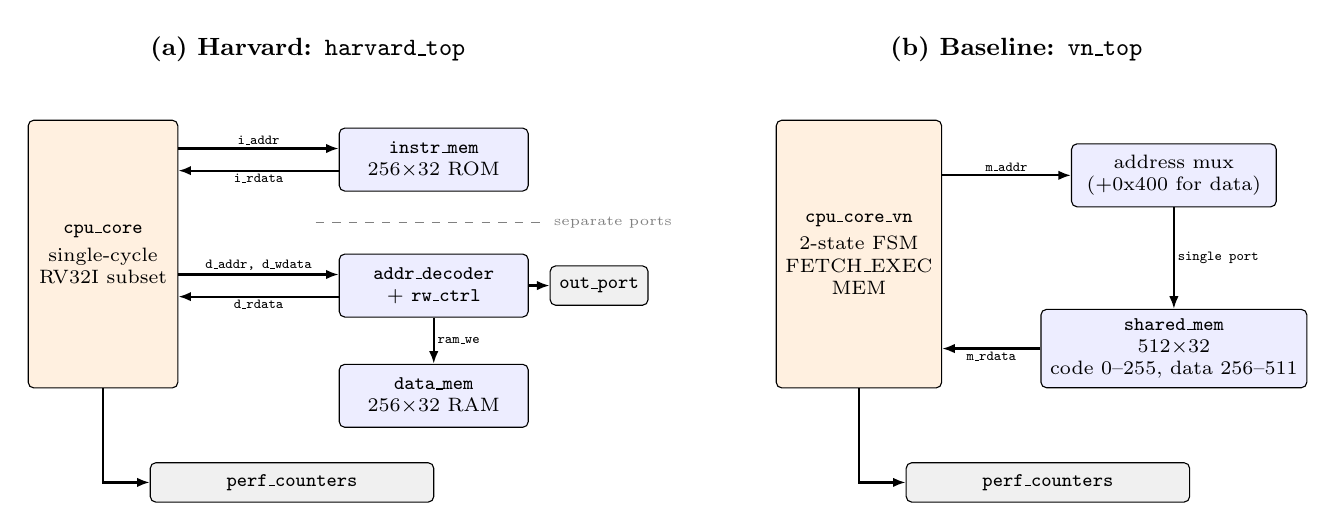
\begin{tikzpicture}[
  font=\scriptsize,
  blk/.style={draw, rounded corners=2pt, align=center, minimum height=0.8cm, fill=blue!7},
  cpu/.style={draw, rounded corners=2pt, align=center, fill=orange!12, minimum width=1.9cm},
  ctr/.style={draw, rounded corners=2pt, align=center, fill=gray!12, minimum height=0.5cm},
  arr/.style={-{Latex[length=1.6mm]}, thick},
  lbl/.style={font=\tiny\ttfamily, fill=white, inner sep=1pt}]

% ---------------- (a) Harvard ----------------
\node[font=\small\bfseries] at (2.6,3.0) {(a) Harvard: \texttt{harvard\_top}};
\node[cpu, minimum height=3.4cm] (core) at (0,0.4) {\texttt{cpu\_core}\\[2pt]single-cycle\\RV32I subset};
\node[blk, minimum width=2.4cm] (imem) at (4.2,1.6) {\texttt{instr\_mem}\\256$\times$32 ROM};
\node[blk, minimum width=2.4cm] (dec)  at (4.2,0.0) {\texttt{addr\_decoder}\\+ \texttt{rw\_ctrl}};
\node[blk, minimum width=2.4cm] (dmem) at (4.2,-1.4) {\texttt{data\_mem}\\256$\times$32 RAM};
\node[ctr] (out) at (6.3,0.0) {\texttt{out\_port}};
\draw[arr] ([yshift=4pt]core.east |- imem.west) -- node[lbl,above]{i\_addr} ([yshift=4pt]imem.west);
\draw[arr] ([yshift=-4pt]imem.west) -- node[lbl,below]{i\_rdata} ([yshift=-4pt]core.east |- imem.west);
\draw[arr] ([yshift=4pt]core.east |- dec.west) -- node[lbl,above]{d\_addr, d\_wdata} ([yshift=4pt]dec.west);
\draw[arr] ([yshift=-4pt]dec.west) -- node[lbl,below]{d\_rdata} ([yshift=-4pt]core.east |- dec.west);
\draw[arr] (dec.south) -- node[lbl,right]{ram\_we} (dmem.north);
\draw[arr] (dec.east) -- (out.west);
\draw[dashed, gray] (2.7,0.8) -- (5.6,0.8) node[right, font=\tiny, text=gray]{separate ports};
\node[ctr, minimum width=3.6cm] (pc) at (2.4,-2.5) {\texttt{perf\_counters}};
\draw[arr] (core.south) |- (pc.west);

% ---------------- (b) Shared memory ----------------
\begin{scope}[xshift=9.6cm]
\node[font=\small\bfseries] at (2.0,3.0) {(b) Baseline: \texttt{vn\_top}};
\node[cpu, minimum height=3.4cm] (vcore) at (0,0.4) {\texttt{cpu\_core\_vn}\\[2pt]2-state FSM\\FETCH\_EXEC\\MEM};
\node[blk, minimum width=2.6cm] (vdec) at (4.0,1.4) {address mux\\(+0x400 for data)};
\node[blk, minimum width=2.6cm] (smem) at (4.0,-0.8) {\texttt{shared\_mem}\\512$\times$32\\code 0--255, data 256--511};
\draw[arr] (vcore.east |- vdec.west) -- node[lbl,above]{m\_addr} (vdec.west);
\draw[arr] (vdec.south) -- node[lbl,right]{single port} (smem.north);
\draw[arr] (smem.west) -- node[lbl,below]{m\_rdata} (vcore.east |- smem.west);
\node[ctr, minimum width=3.6cm] (vpc) at (2.4,-2.5) {\texttt{perf\_counters}};
\draw[arr] (vcore.south) |- (vpc.west);
\end{scope}
\end{tikzpicture}
}
  \caption{Phase I. (a) Harvard system: the processor reaches the instruction ROM and the data
  side through separate ports. (b) Shared-memory baseline: fetches and data accesses use one
  port to a single memory.}
  \label{fig:block1}
\end{figure*}

\begin{figure}[t]
  \centering
  \resizebox{0.62\columnwidth}{!}{% Two-state controller of the shared-memory baseline (Fig. 3)
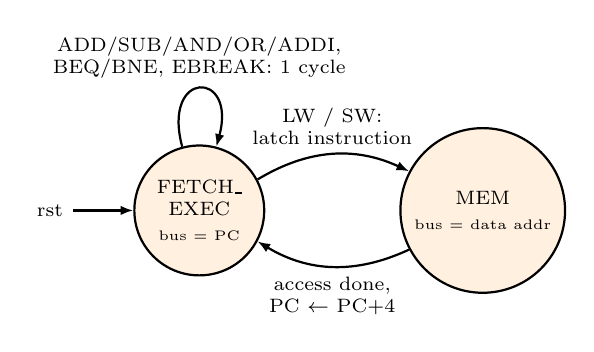
\begin{tikzpicture}[
  font=\scriptsize,
  st/.style={draw, circle, thick, fill=orange!12, minimum size=1.55cm, align=center},
  w/.style={-{Latex[length=1.6mm]}, thick}]
\node[st] (fe) at (0,0) {FETCH\_\\EXEC\\[1pt]{\tiny bus = PC}};
\node[st] (me) at (3.6,0) {MEM\\[1pt]{\tiny bus = data addr}};
\draw[w] (-1.6,0) node[left]{rst} -- (fe);
\draw[w] (fe) to[loop above, looseness=6] node[above, align=center]{ADD/SUB/AND/OR/ADDI,\\BEQ/BNE, EBREAK: 1 cycle} (fe);
\draw[w] (fe) to[bend left=28] node[above, align=center]{LW / SW:\\latch instruction} (me);
\draw[w] (me) to[bend left=28] node[below, align=center]{access done,\\PC $\leftarrow$ PC+4} (fe);
\end{tikzpicture}
}
  \caption{Two-state controller of the single-bus core (Phase I, kept in Phase II).}
  \label{fig:fsm}
\end{figure}

\subsection{Phase II architecture}
Phase~II keeps both processors and puts a memory hierarchy behind them
(Fig.~\ref{fig:block2}). Every Phase~II system uses the same lower-level memory,
\sig{main\_mem}, a single-port memory that holds code at physical addresses
\texttt{0x000}--\texttt{0x3FF} and data at \texttt{0x400}--\texttt{0x7FF} (the Phase~I baseline
layout) and answers each request after $L$ cycles. We compare three organisations:
\begin{itemize}
  \item \textbf{Modified Harvard} (\sig{mh\_top}): \sig{cpu\_core} with an $N$-line
        instruction cache and an $N$-line data cache, which share \sig{main\_mem} through an
        arbiter.
  \item \textbf{Unified cache}: \sig{cpu\_core\_vn} with one cache of $2N$ lines, the same
        total capacity (\sig{vnc\_top} with \sig{CACHE\_EN}\,=\,1).
  \item \textbf{No cache}: \sig{cpu\_core\_vn} with every access going to \sig{main\_mem}
        (\sig{vnc\_top} with \sig{CACHE\_EN}\,=\,0). With $L=1$ it is the Phase~I baseline,
        cycle for cycle.
\end{itemize}
The Phase~I \sig{harvard\_top}, which has ideal single-cycle memories, remains the reference.
In both Phase~II tops the address decoder sends only data-RAM accesses to a cache.
\sig{out\_port} and invalid addresses bypass the caches and finish in their own cycle.

\begin{figure*}[t]
  \centering
  \resizebox{0.80\textwidth}{!}{% Phase II block diagrams: (a) modified Harvard (mh_top), (b) single bus (vnc_top)
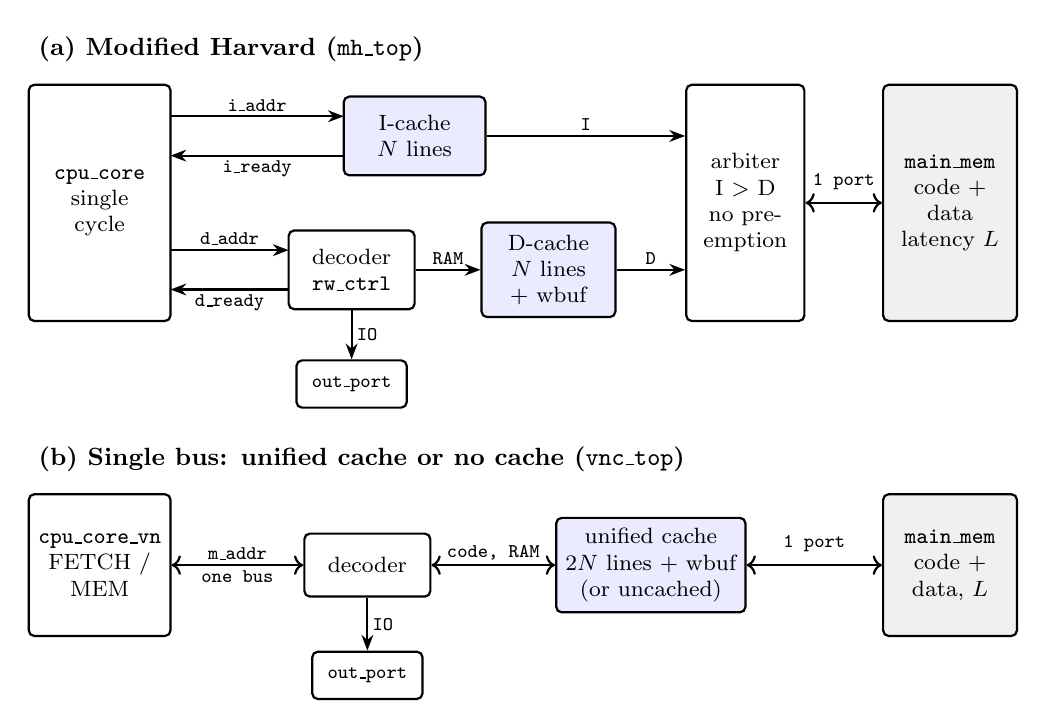
\begin{tikzpicture}[
    font=\footnotesize,
    blk/.style={draw, thick, rounded corners=2pt, minimum height=8mm, align=center, fill=white},
    mem/.style={blk, fill=gray!12},
    cac/.style={blk, fill=blue!8},
    arr/.style={-{Stealth[length=2mm]}, thick},
    lbl/.style={font=\scriptsize\ttfamily, inner sep=1.5pt}]
  % ---------------- (a) modified Harvard ----------------
  \node[blk, minimum width=18mm, minimum height=30mm] (core) at (0,0) {\sig{cpu\_core}\\single\\cycle};
  \node[cac, minimum width=18mm, minimum height=10mm] (ic) at (4.0,0.85) {I-cache\\$N$ lines};
  \node[blk, minimum width=16mm, minimum height=10mm] (dec) at (3.2,-0.85) {decoder\\\sig{rw\_ctrl}};
  \node[cac, minimum width=17mm, minimum height=12mm] (dc) at (5.7,-0.85) {D-cache\\$N$ lines\\+ wbuf};
  \node[blk, minimum width=15mm, minimum height=30mm] (arb) at (8.2,0) {arbiter\\I $>$ D\\no pre-\\emption};
  \node[mem, minimum width=17mm, minimum height=30mm] (mm) at (10.8,0) {\sig{main\_mem}\\code +\\data\\latency $L$};
  \node[blk, minimum width=14mm, minimum height=6mm, font=\scriptsize] (io) at (3.2,-2.3) {\sig{out\_port}};
  \draw[arr] (0.9,1.10) -- node[lbl, above] {i\_addr} (3.1,1.10);
  \draw[arr] (3.1,0.60) -- node[lbl, below] {i\_ready} (0.9,0.60);
  \draw[arr] (0.9,-0.60) -- node[lbl, above] {d\_addr} (2.4,-0.60);
  \draw[arr] (2.4,-1.10) -- node[lbl, below] {d\_ready} (0.9,-1.10);
  \draw[arr] (dec.east) -- node[lbl, above] {RAM} (dc.west);
  \draw[arr] (dec.south) -- node[lbl, right] {IO} (io.north);
  \draw[arr] (ic.east) -- node[lbl, above] {I} (ic.east -| arb.west);
  \draw[arr] (dc.east) -- node[lbl, above] {D} (dc.east -| arb.west);
  \draw[arr, <->] (arb.east) -- node[lbl, above=3pt] {1 port} (mm.west);
  \node[font=\small\bfseries, anchor=west] at (-0.9,1.95) {(a) Modified Harvard (\sig{mh\_top})};
  % ---------------- (b) single bus ----------------
  \begin{scope}[yshift=-4.6cm]
    \node[blk, minimum width=18mm, minimum height=18mm] (vcore) at (0,0) {\sig{cpu\_core\_vn}\\FETCH /\\MEM};
    \node[blk, minimum width=16mm] (vdec) at (3.4,0) {decoder};
    \node[cac, minimum width=24mm, minimum height=12mm] (uc) at (7.0,0) {unified cache\\$2N$ lines + wbuf\\(or uncached)};
    \node[mem, minimum width=17mm, minimum height=18mm] (vmm) at (10.8,0) {\sig{main\_mem}\\code +\\data, $L$};
    \node[blk, minimum width=14mm, minimum height=6mm, font=\scriptsize] (vio) at (3.4,-1.4) {\sig{out\_port}};
    \draw[arr, <->] (vcore.east) -- node[lbl, above] {m\_addr} node[lbl, below] {one bus} (vdec.west);
    \draw[arr, <->] (vdec.east) -- node[lbl, above] {code, RAM} (uc.west);
    \draw[arr] (vdec.south) -- node[lbl, right] {IO} (vio.north);
    \draw[arr, <->] (uc.east) -- node[lbl, above=3pt] {1 port} (vmm.west);
    \node[font=\small\bfseries, anchor=west] at (-0.9,1.35) {(b) Single bus: unified cache or no cache (\sig{vnc\_top})};
  \end{scope}
\end{tikzpicture}
}
  \caption{Phase II. (a) Modified Harvard: split L1 caches over one shared memory, with an
  arbiter giving instruction refills priority. (b) Single bus: the same memory behind a unified
  cache of twice the size, or behind no cache. Both systems use the same cache module and the
  same \sig{main\_mem}.}
  \label{fig:block2}
\end{figure*}

\subsection{Processor extensions}
To run realistic programs, both processors gained XOR, SLT, SLL and SRL, their immediate forms
XORI, SLTI, SLLI and SRLI, the branches BLT and BGE, the jumps JAL and JALR, and LUI, all with
standard RV32I encodings \cite{riscv_spec}. The ALU gained four operations (XOR, signed
set-less-than, and the two logical shifts by \sig{b[4:0]}). BLT and BGE reuse the zero flag after
an SLT, the way BEQ and BNE use it after a SUB. JAL and JALR write $\mathrm{PC}+4$, LUI writes the
U-immediate, and the immediate generator gained the U and J formats. The decoder keeps every
Phase~I output with its old meaning, so the Phase~I subset decodes exactly as before.

Each core also gained a stall interface:
\begin{itemize}
  \item \sig{i\_ready}\,=\,0 (\sig{cpu\_core}): no valid instruction yet. The core decodes a
        NOP, so nothing is written or accessed, and holds its PC.
  \item \sig{d\_ready}\,=\,0 (\sig{cpu\_core}): the load or store of this cycle has not
        finished. The PC and register file are held and the data request stays on the port.
  \item \sig{m\_ready}\,=\,0 (\sig{cpu\_core\_vn}): the bus transfer has not finished. The
        state, PC, latched instruction and register file are held.
\end{itemize}
The Phase~I top levels tie these inputs to 1. With them tied, the enable equations reduce to the
Phase~I ones, and re-running the Phase~I regression gives byte-identical logs: every Phase~I
cycle count is unchanged.

\subsection{Timing design rules}
Every path from the memory back to the processor must end in a register. Otherwise the system
contains a combinational loop, which a static timing tool cannot analyse. We followed two rules:
\begin{enumerate}
  \item \textbf{No forwarding of refill data.} When a miss is served, the cache writes the line
        into its array and answers as a hit in the \emph{next} cycle. If the refill data went
        straight to the core, it would feed the decoder, the ALU, the next data address, the
        D-cache request and the arbiter's address multiplexer, and so reach the memory input
        again.
  \item \textbf{The I-cache request is \sig{\textasciitilde halted}, a register.} If it were
        \sig{\textasciitilde halt}, which also depends on the EBREAK decoded from the fetched
        word, the request would depend on the cache's own output.
\end{enumerate}
Section~\ref{sec:area} shows that the modified Harvard design synthesises with no loop warning,
and that copies which break either rule produce loops.

% Owner: Yashpal (Member 1)
\subsection{Reusable cache}
One module, \sig{cache}, serves as the I-cache, the D-cache and the unified cache
(Fig.~\ref{fig:cache}). It is direct-mapped, with \sig{NUM\_LINES} lines of \sig{LINE\_WORDS}
32-bit words (both powers of two), one valid bit and one tag per line. The fields are computed
with shifts and masks, so a one-line cache or a one-word line also works. All results use
4-word lines.
\begin{itemize}
  \item \textbf{Read hit:} completes in the same cycle through a combinational array read.
  \item \textbf{Read miss:} requests the whole line, writes it into the array in the cycle the
        memory answers, and completes as a hit in the next cycle. The miss penalty is
        therefore exactly $L$ cycles. A read miss first waits for the write buffer to drain,
        so the line it fetches already contains any buffered store (no read-after-write
        hazard).
  \item \textbf{Writes:} write-through and no-write-allocate. A store hit also updates the
        word in the line. A store miss leaves the cache unchanged.
  \item \textbf{Write buffer} (\sig{WBUF}\,=\,1): one entry. A store that finds the buffer
        empty is offered to memory at once. If memory does not finish it in that cycle, the
        buffer captures it and keeps the same request asserted, so the latency count simply
        continues while the core goes on. A store that finds the buffer busy waits until it
        empties. With $L=1$ the buffer is therefore never used, and a store is never slower
        than without the buffer. Without the buffer a store waits for memory.
  \item \textbf{Uncached mode} (\sig{ENABLE}\,=\,0): every read goes to memory and its word is
        passed straight back. With $L=1$ this is the Phase~I combinational memory.
\end{itemize}
The cache also outputs event pulses for refills and write-buffer stalls, which the performance
counters use.

\begin{figure}[t]
  \centering
  \resizebox{0.92\columnwidth}{!}{% Organisation of the reusable direct-mapped cache (rtl/mem/cache.v)
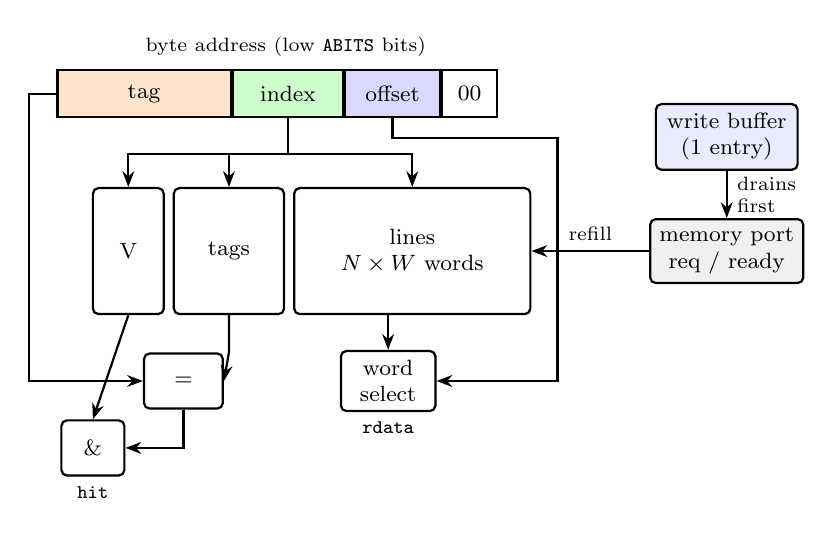
\begin{tikzpicture}[
    font=\footnotesize,
    fld/.style={draw, thick, minimum height=6mm, align=center, inner sep=2pt},
    blk/.style={draw, thick, rounded corners=2pt, minimum height=7mm, align=center, fill=white},
    arr/.style={-{Stealth[length=2mm]}, thick}]
  % address fields
  \node[fld, minimum width=22mm, fill=orange!20] (tag) at (0,0) {tag};
  \node[fld, minimum width=14mm, fill=green!20, right=0mm of tag] (idx) {index};
  \node[fld, minimum width=12mm, fill=blue!15, right=0mm of idx] (off) {offset};
  \node[fld, minimum width=7mm, right=0mm of off] (bb) {00};
  \node[anchor=south, font=\scriptsize] at (1.8,0.35) {byte address (low \sig{ABITS} bits)};
  % arrays
  \node[blk, minimum width=9mm, minimum height=16mm] (v) at (-0.2,-2.0) {V};
  \node[blk, minimum width=14mm, minimum height=16mm, right=1mm of v] (t) {tags};
  \node[blk, minimum width=30mm, minimum height=16mm, right=1mm of t] (d) {lines\\$N \times W$ words};
  \draw[arr] (idx.south) -- ++(0,-0.45) -| (t.north);
  \draw[arr] (idx.south) ++(0,-0.45) -| (d.north);
  \draw[arr] (idx.south) ++(0,-0.45) -| (v.north);
  \node[blk, minimum width=10mm] (cmp) at (0.5,-3.65) {$=$};
  \draw[arr] (t.south) -- (cmp.north -| t.south) -- (cmp.east);
  \draw[arr] (tag.west) -- ++(-0.35,0) |- (cmp.west);
  \node[blk, minimum width=8mm] (and) at (-0.65,-4.5) {\&};
  \draw[arr] (v.south) -- (and.north);
  \draw[arr] (cmp.south) |- (and.east);
  \node[anchor=north, font=\scriptsize\ttfamily] at (and.south) {hit};
  \node[blk, minimum width=12mm] (mux) at (3.1,-3.65) {word\\select};
  \draw[arr] (d.south -| mux.north) -- (mux.north);
  \draw[arr] (off.south) -- ++(0,-0.25) -| (5.25,-3.65) -- (mux.east);
  \node[anchor=north, font=\scriptsize\ttfamily] at (mux.south) {rdata};
  % write buffer and memory side
  \node[blk, minimum width=18mm, fill=blue!8] (wb) at (7.4,-0.55) {write buffer\\(1 entry)};
  \node[blk, minimum width=18mm, fill=gray!12] (mp) at (7.4,-2.0) {memory port\\req / ready};
  \draw[arr] (wb) -- node[right, font=\scriptsize, align=left] {drains\\first} (mp);
  \draw[arr] (mp.west) -- node[above, font=\scriptsize] {refill} (d.east |- mp.west);
\end{tikzpicture}
}
  \caption{The reusable direct-mapped cache: address fields, valid/tag/line arrays, hit logic,
  word select, and the one-entry write buffer in front of the memory port.}
  \label{fig:cache}
\end{figure}

\subsection{Shared lower-level memory}
\sig{main\_mem} is a 512-word single-port memory. A requester raises \sig{req} with
\sig{we}, \sig{addr} and \sig{wdata} and holds them until \sig{ready}, which rises in the $L$-th
cycle of the request. A read returns the aligned 4-word line that contains \sig{addr}, so a
refill is one transfer. A write stores one word. With $L=1$, \sig{ready} rises in the same cycle
as \sig{req}, which is exactly the ideal memory of Phase~I. In synthesis the memory is a black
box that stands for block RAM or off-chip memory.

% Owner: Ankit (Member 3)
\subsection{Arbiter and system tops}
In the modified Harvard system both caches refill from the same memory, so \sig{arbiter} decides
who uses the port. Instruction requests have fixed priority, because the core can do nothing
without its next instruction. Once a transfer has started, it is never pre-empted: a register
remembers the owner until \sig{ready}. Otherwise the memory's latency count would be handed to
the other request. The grant depends only on the two requests and that register, and nothing is
forwarded from memory into a request, so the arbiter adds no combinational loop. A
\emph{conflict cycle} is a cycle in which both caches request the memory. Since the core is
single-cycle, an instruction miss and a data access cannot normally happen at the same time:
while the I-cache misses, the core executes a NOP. Conflicts therefore arise only when the write
buffer is still draining a store as the next instruction misses.

\sig{mh\_top} connects the core, the I-cache (no write buffer), the Phase~I \sig{addr\_decoder}
and \sig{rw\_ctrl}, the D-cache at physical address \sig{d\_addr}\,$+$\,\texttt{0x400}, the
arbiter and \sig{main\_mem}. \sig{vnc\_top} connects the single-bus core to the same decoder,
one cache (unified, or uncached) and \sig{main\_mem}. Fetches use the PC unchanged, and data-RAM
accesses add \texttt{0x400}, as in Phase~I.

\subsection{Performance counters}
The Phase~I \sig{perf\_counters} (cycles, retired instructions, completed data accesses) is
used unchanged. A new \sig{event\_counters} module counts I-misses, D-misses, I-stall cycles,
D-stall cycles, write-buffer stall cycles and arbiter conflict cycles, and follows the same
freeze rule: the EBREAK cycle is counted, then every counter stops. These counters make exact
cycle-accounting identities possible:
\begin{align}
  \text{cycles}_{\text{mH}} &= I + S_I + S_D, \label{eq:mh}\\
  \text{cycles}_{\text{bus}} &= I + A + S_I + S_D, \label{eq:bus}
\end{align}
where $I$ is the number of retired instructions, $A$ the number of loads and stores (the extra
\textsc{Mem} cycle of the single bus), and $S_I$, $S_D$ the instruction and data stall cycles.

% Owner: Samriddhi (Member 4)
\subsection{Verification approach}
The RTL is Verilog-2001 \cite{ieee1364}, simulated with Icarus Verilog \cite{icarus}. Every
testbench checks its own results and prints \texttt{PASS} or \texttt{FAIL}, and one
\sig{Makefile} runs the whole flow (\texttt{make all}).

\textbf{Assembler and programs.} The Phase~I two-pass assembler now supports the new
instructions and the pseudo-instructions \texttt{j}, \texttt{ret} and \texttt{mv}. Its
self-test checks 29 encodings against hand-computed values, including well-known reference
encodings such as \texttt{ret}\,=\,\texttt{0x00008067}. Four new programs, each with different
memory behaviour, join the Phase~I four:
\begin{itemize}
  \item \sig{bubble\_sort}: sorts 16 signed words. It has strong temporal locality and issues
        stores in pairs, one pair per swap.
  \item \sig{subroutine}: multiply, GCD and popcount subroutines and a nested call through a
        stack. Its 59-word code footprint exceeds an 8-line instruction cache.
  \item \sig{transpose}: an $8\times8$ matrix transpose. Its reads are sequential (spatial
        locality) and its writes have a stride of 8 words.
  \item \sig{isa\_test}: every new instruction once, with hand-computed results.
\end{itemize}
The final register and memory values of every program were worked out by hand (and with plain
Python) and are checked on both Phase~I systems.

\textbf{Golden model.} \sig{tools/iss.py} is an instruction-set simulator written independently
of the RTL and the assembler. It decodes the instruction bits itself. It predicts the final
registers, data memory and \sig{out\_port}; the instruction, load and store counts; and the
misses of split and unified direct-mapped caches of any size, with write-through and
no-write-allocate.

\textbf{Cache unit test.} \sig{tb\_cache} drives four caches with memories of latency 3 or 1.
Its 41 checks cover miss timing ($1+L$ cycles), hits, a buffered store, a store waiting for a
busy buffer, no-write-allocate, a read after a buffered store miss, conflict eviction, store
hits with and without a buffer, and uncached mode. We confirmed that the test can fail by
running it against three deliberately broken copies of the RTL: one with the read-after-write
wait removed, one where a store miss writes the line, and one with an off-by-one memory latency.
Each copy fails at least one check (\texttt{make mutate}).

\textbf{System testbench.} \sig{tb\_system} runs one program on five systems at once: the ideal
Harvard reference, the modified Harvard system, the unified-cache system, the no-cache system
and the Phase~I baseline. It checks that:
\begin{itemize}
  \item registers, all 256 data words, \sig{out\_port}, instruction counts, data-access counts
        and fault cycles match the reference;
  \item the identities (\ref{eq:mh})--(\ref{eq:bus}) hold;
  \item there are no conflicts on a single bus, and no conflicts or write-buffer stalls when the
        buffer is off;
  \item with $L=1$, the no-cache system equals the Phase~I baseline in cycle count and in bus
        address and FSM state in every cycle.
\end{itemize}

\textbf{Sweep.} \sig{tools/sweep.py} runs \sig{tb\_system} for eight programs
$\times$ $L\in\{1,2,4,8,16\}$ $\times$ $N\in\{1,2,4,8,16,32\}$ lines per split cache
$\times$ write buffer off/on, plus a placement experiment (Section~\ref{sec:split}): 528 runs in
all. It cross-checks every RTL miss count and instruction count against the golden model, and
every final state against the ISS. With the buffer off it also checks an exact stall model.
Cached systems must satisfy $S_I = L\cdot M_I$ and $S_D = L\cdot M_D + (L-1)\cdot W$. The
no-cache system must satisfy $S_I = (L-1)\cdot I$ and $S_D=(L-1)(R+W)$. Here $M$ is a miss count
and $R$, $W$ are the loads and stores to RAM. All 528 runs pass, with 9888 golden-model checks
and no mismatch. The script also writes the CSV file, the summary tables and the plot data used
below, so no number in this report was typed by hand.


% Owner: Ankit (Member 3)
%=====================================================================
\section{Results and Discussion}
%=====================================================================
\subsection{Phase I: ideal Harvard vs shared memory}
Table~\ref{tab:p1} lists the two Phase~I systems, now running the extended instruction set; all
tests pass. The first four rows are identical to the Phase~I report, which confirms that the
extension did not change Phase~I timing. The Harvard system always runs at CPI\,=\,1.00, and
every one of its data accesses overlaps a fetch. The baseline needs exactly one extra cycle per
load or store, so
\begin{equation}
  \mathrm{CPI}_{\text{baseline}} = 1 + f_{\text{LS}},
\end{equation}
where $f_{\text{LS}}$ is the fraction of instructions that are loads or stores. The speed-up
grows with memory intensity, from 1.02$\times$ for \sig{count\_loop} to 1.42$\times$ for
\sig{isa\_test}. Fig.~\ref{fig:wave1} shows the effect cycle by cycle.

\begin{table}[t]
  \caption{Ideal memories: Harvard vs single-port baseline (Icarus Verilog)}
  \label{tab:p1}
  \centering
  \setlength{\tabcolsep}{3.2pt}
  \begin{tabular}{@{}lrrrrrr@{}}
    \toprule
    Program & Instr & LS\% & Harv.\ cyc & Base.\ cyc & Base.\ CPI & Speed-up \\
    \midrule
    \tabinput{data/tab_phase1.tex}
    \bottomrule
  \end{tabular}
\end{table}

\begin{figure*}[t]
  \centering
  \resizebox{0.80\textwidth}{!}{% generated by tools/vcd2tikz.py from tb_compare_memcopy.vcd -- do not edit
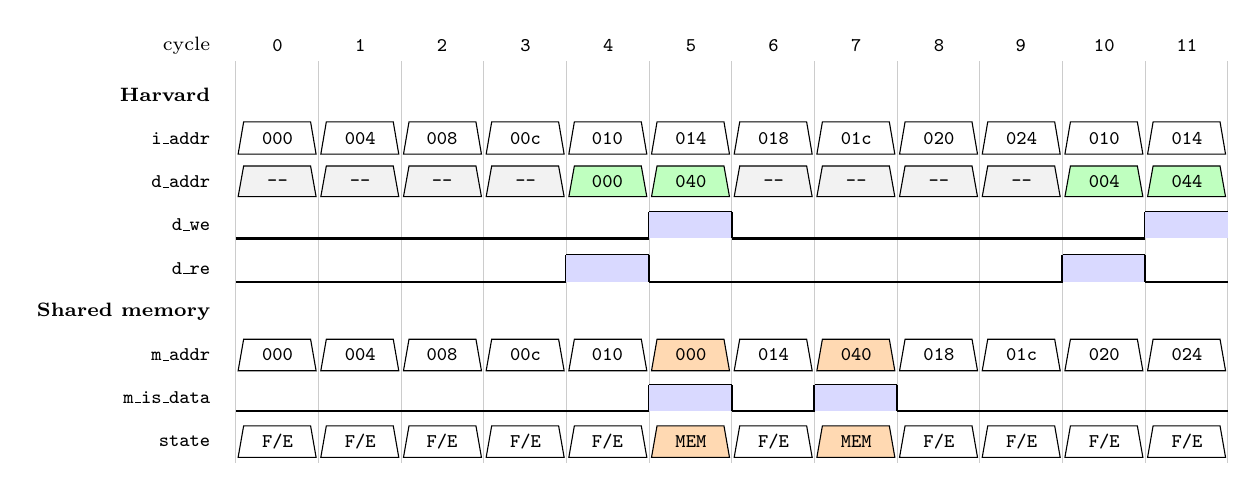
\begin{tikzpicture}[font=\scriptsize\ttfamily, x=1cm, y=1cm]
\node at (0.53,0.35) {0};
\node at (1.58,0.35) {1};
\node at (2.62,0.35) {2};
\node at (3.68,0.35) {3};
\node at (4.73,0.35) {4};
\node at (5.78,0.35) {5};
\node at (6.83,0.35) {6};
\node at (7.88,0.35) {7};
\node at (8.93,0.35) {8};
\node at (9.97,0.35) {9};
\node at (11.03,0.35) {10};
\node at (12.08,0.35) {11};
\node[anchor=east] at (-0.2,0.35) {\normalfont cycle};
\draw[gray!40] (0.00,0.15) -- (0.00,-4.95);
\draw[gray!40] (1.05,0.15) -- (1.05,-4.95);
\draw[gray!40] (2.10,0.15) -- (2.10,-4.95);
\draw[gray!40] (3.15,0.15) -- (3.15,-4.95);
\draw[gray!40] (4.20,0.15) -- (4.20,-4.95);
\draw[gray!40] (5.25,0.15) -- (5.25,-4.95);
\draw[gray!40] (6.30,0.15) -- (6.30,-4.95);
\draw[gray!40] (7.35,0.15) -- (7.35,-4.95);
\draw[gray!40] (8.40,0.15) -- (8.40,-4.95);
\draw[gray!40] (9.45,0.15) -- (9.45,-4.95);
\draw[gray!40] (10.50,0.15) -- (10.50,-4.95);
\draw[gray!40] (11.55,0.15) -- (11.55,-4.95);
\draw[gray!40] (12.60,0.15) -- (12.60,-4.95);
\node[anchor=east,font=\normalfont\bfseries\scriptsize] at (-0.2,-0.28) {Harvard};
\node[anchor=east] at (-0.2,-0.83) {i\_addr};
\draw[fill=white] (0.03,-1.03) -- (0.10,-0.62) -- (0.95,-0.62) -- (1.02,-1.03) -- cycle;
\node at (0.53,-0.83) {000};
\draw[fill=white] (1.08,-1.03) -- (1.15,-0.62) -- (2.00,-0.62) -- (2.07,-1.03) -- cycle;
\node at (1.58,-0.83) {004};
\draw[fill=white] (2.13,-1.03) -- (2.20,-0.62) -- (3.05,-0.62) -- (3.12,-1.03) -- cycle;
\node at (2.62,-0.83) {008};
\draw[fill=white] (3.18,-1.03) -- (3.25,-0.62) -- (4.10,-0.62) -- (4.17,-1.03) -- cycle;
\node at (3.68,-0.83) {00c};
\draw[fill=white] (4.23,-1.03) -- (4.30,-0.62) -- (5.15,-0.62) -- (5.22,-1.03) -- cycle;
\node at (4.72,-0.83) {010};
\draw[fill=white] (5.28,-1.03) -- (5.35,-0.62) -- (6.20,-0.62) -- (6.27,-1.03) -- cycle;
\node at (5.78,-0.83) {014};
\draw[fill=white] (6.33,-1.03) -- (6.40,-0.62) -- (7.25,-0.62) -- (7.32,-1.03) -- cycle;
\node at (6.83,-0.83) {018};
\draw[fill=white] (7.38,-1.03) -- (7.45,-0.62) -- (8.30,-0.62) -- (8.37,-1.03) -- cycle;
\node at (7.88,-0.83) {01c};
\draw[fill=white] (8.43,-1.03) -- (8.50,-0.62) -- (9.35,-0.62) -- (9.42,-1.03) -- cycle;
\node at (8.93,-0.83) {020};
\draw[fill=white] (9.48,-1.03) -- (9.55,-0.62) -- (10.40,-0.62) -- (10.47,-1.03) -- cycle;
\node at (9.98,-0.83) {024};
\draw[fill=white] (10.53,-1.03) -- (10.60,-0.62) -- (11.45,-0.62) -- (11.52,-1.03) -- cycle;
\node at (11.03,-0.83) {010};
\draw[fill=white] (11.58,-1.03) -- (11.65,-0.62) -- (12.50,-0.62) -- (12.57,-1.03) -- cycle;
\node at (12.08,-0.83) {014};
\node[anchor=east] at (-0.2,-1.38) {d\_addr};
\draw[fill=gray!10] (0.03,-1.57) -- (0.10,-1.18) -- (0.95,-1.18) -- (1.02,-1.57) -- cycle;
\node at (0.53,-1.38) {--};
\draw[fill=gray!10] (1.08,-1.57) -- (1.15,-1.18) -- (2.00,-1.18) -- (2.07,-1.57) -- cycle;
\node at (1.58,-1.38) {--};
\draw[fill=gray!10] (2.13,-1.57) -- (2.20,-1.18) -- (3.05,-1.18) -- (3.12,-1.57) -- cycle;
\node at (2.62,-1.38) {--};
\draw[fill=gray!10] (3.18,-1.57) -- (3.25,-1.18) -- (4.10,-1.18) -- (4.17,-1.57) -- cycle;
\node at (3.68,-1.38) {--};
\draw[fill=green!25] (4.23,-1.57) -- (4.30,-1.18) -- (5.15,-1.18) -- (5.22,-1.57) -- cycle;
\node at (4.72,-1.38) {000};
\draw[fill=green!25] (5.28,-1.57) -- (5.35,-1.18) -- (6.20,-1.18) -- (6.27,-1.57) -- cycle;
\node at (5.78,-1.38) {040};
\draw[fill=gray!10] (6.33,-1.57) -- (6.40,-1.18) -- (7.25,-1.18) -- (7.32,-1.57) -- cycle;
\node at (6.83,-1.38) {--};
\draw[fill=gray!10] (7.38,-1.57) -- (7.45,-1.18) -- (8.30,-1.18) -- (8.37,-1.57) -- cycle;
\node at (7.88,-1.38) {--};
\draw[fill=gray!10] (8.43,-1.57) -- (8.50,-1.18) -- (9.35,-1.18) -- (9.42,-1.57) -- cycle;
\node at (8.93,-1.38) {--};
\draw[fill=gray!10] (9.48,-1.57) -- (9.55,-1.18) -- (10.40,-1.18) -- (10.47,-1.57) -- cycle;
\node at (9.98,-1.38) {--};
\draw[fill=green!25] (10.53,-1.57) -- (10.60,-1.18) -- (11.45,-1.18) -- (11.52,-1.57) -- cycle;
\node at (11.03,-1.38) {004};
\draw[fill=green!25] (11.58,-1.57) -- (11.65,-1.18) -- (12.50,-1.18) -- (12.57,-1.57) -- cycle;
\node at (12.08,-1.38) {044};
\node[anchor=east] at (-0.2,-1.93) {d\_we};
\draw[thick] (0.00,-2.10) -- (1.05,-2.10);
\draw[thick] (1.05,-2.10) -- (2.10,-2.10);
\draw[thick] (2.10,-2.10) -- (3.15,-2.10);
\draw[thick] (3.15,-2.10) -- (4.20,-2.10);
\draw[thick] (4.20,-2.10) -- (5.25,-2.10);
\draw[thick] (5.25,-1.76) -- (6.30,-1.76);
\draw[thick] (5.25,-2.10) -- (5.25,-1.76);
\fill[blue!15] (5.25,-2.10) rectangle (6.30,-1.76);
\draw[thick] (6.30,-2.10) -- (7.35,-2.10);
\draw[thick] (6.30,-2.10) -- (6.30,-1.76);
\draw[thick] (7.35,-2.10) -- (8.40,-2.10);
\draw[thick] (8.40,-2.10) -- (9.45,-2.10);
\draw[thick] (9.45,-2.10) -- (10.50,-2.10);
\draw[thick] (10.50,-2.10) -- (11.55,-2.10);
\draw[thick] (11.55,-1.76) -- (12.60,-1.76);
\draw[thick] (11.55,-2.10) -- (11.55,-1.76);
\fill[blue!15] (11.55,-2.10) rectangle (12.60,-1.76);
\node[anchor=east] at (-0.2,-2.48) {d\_re};
\draw[thick] (0.00,-2.65) -- (1.05,-2.65);
\draw[thick] (1.05,-2.65) -- (2.10,-2.65);
\draw[thick] (2.10,-2.65) -- (3.15,-2.65);
\draw[thick] (3.15,-2.65) -- (4.20,-2.65);
\draw[thick] (4.20,-2.31) -- (5.25,-2.31);
\draw[thick] (4.20,-2.65) -- (4.20,-2.31);
\fill[blue!15] (4.20,-2.65) rectangle (5.25,-2.31);
\draw[thick] (5.25,-2.65) -- (6.30,-2.65);
\draw[thick] (5.25,-2.65) -- (5.25,-2.31);
\draw[thick] (6.30,-2.65) -- (7.35,-2.65);
\draw[thick] (7.35,-2.65) -- (8.40,-2.65);
\draw[thick] (8.40,-2.65) -- (9.45,-2.65);
\draw[thick] (9.45,-2.65) -- (10.50,-2.65);
\draw[thick] (10.50,-2.31) -- (11.55,-2.31);
\draw[thick] (10.50,-2.65) -- (10.50,-2.31);
\fill[blue!15] (10.50,-2.65) rectangle (11.55,-2.31);
\draw[thick] (11.55,-2.65) -- (12.60,-2.65);
\draw[thick] (11.55,-2.65) -- (11.55,-2.31);
\node[anchor=east,font=\normalfont\bfseries\scriptsize] at (-0.2,-3.03) {Shared memory};
\node[anchor=east] at (-0.2,-3.58) {m\_addr};
\draw[fill=white] (0.03,-3.78) -- (0.10,-3.38) -- (0.95,-3.38) -- (1.02,-3.78) -- cycle;
\node at (0.53,-3.58) {000};
\draw[fill=white] (1.08,-3.78) -- (1.15,-3.38) -- (2.00,-3.38) -- (2.07,-3.78) -- cycle;
\node at (1.58,-3.58) {004};
\draw[fill=white] (2.13,-3.78) -- (2.20,-3.38) -- (3.05,-3.38) -- (3.12,-3.78) -- cycle;
\node at (2.62,-3.58) {008};
\draw[fill=white] (3.18,-3.78) -- (3.25,-3.38) -- (4.10,-3.38) -- (4.17,-3.78) -- cycle;
\node at (3.68,-3.58) {00c};
\draw[fill=white] (4.23,-3.78) -- (4.30,-3.38) -- (5.15,-3.38) -- (5.22,-3.78) -- cycle;
\node at (4.72,-3.58) {010};
\draw[fill=orange!30] (5.28,-3.78) -- (5.35,-3.38) -- (6.20,-3.38) -- (6.27,-3.78) -- cycle;
\node at (5.78,-3.58) {000};
\draw[fill=white] (6.33,-3.78) -- (6.40,-3.38) -- (7.25,-3.38) -- (7.32,-3.78) -- cycle;
\node at (6.83,-3.58) {014};
\draw[fill=orange!30] (7.38,-3.78) -- (7.45,-3.38) -- (8.30,-3.38) -- (8.37,-3.78) -- cycle;
\node at (7.88,-3.58) {040};
\draw[fill=white] (8.43,-3.78) -- (8.50,-3.38) -- (9.35,-3.38) -- (9.42,-3.78) -- cycle;
\node at (8.93,-3.58) {018};
\draw[fill=white] (9.48,-3.78) -- (9.55,-3.38) -- (10.40,-3.38) -- (10.47,-3.78) -- cycle;
\node at (9.98,-3.58) {01c};
\draw[fill=white] (10.53,-3.78) -- (10.60,-3.38) -- (11.45,-3.38) -- (11.52,-3.78) -- cycle;
\node at (11.03,-3.58) {020};
\draw[fill=white] (11.58,-3.78) -- (11.65,-3.38) -- (12.50,-3.38) -- (12.57,-3.78) -- cycle;
\node at (12.08,-3.58) {024};
\node[anchor=east] at (-0.2,-4.12) {m\_is\_data};
\draw[thick] (0.00,-4.29) -- (1.05,-4.29);
\draw[thick] (1.05,-4.29) -- (2.10,-4.29);
\draw[thick] (2.10,-4.29) -- (3.15,-4.29);
\draw[thick] (3.15,-4.29) -- (4.20,-4.29);
\draw[thick] (4.20,-4.29) -- (5.25,-4.29);
\draw[thick] (5.25,-3.96) -- (6.30,-3.96);
\draw[thick] (5.25,-4.29) -- (5.25,-3.96);
\fill[blue!15] (5.25,-4.29) rectangle (6.30,-3.96);
\draw[thick] (6.30,-4.29) -- (7.35,-4.29);
\draw[thick] (6.30,-4.29) -- (6.30,-3.96);
\draw[thick] (7.35,-3.96) -- (8.40,-3.96);
\draw[thick] (7.35,-4.29) -- (7.35,-3.96);
\fill[blue!15] (7.35,-4.29) rectangle (8.40,-3.96);
\draw[thick] (8.40,-4.29) -- (9.45,-4.29);
\draw[thick] (8.40,-4.29) -- (8.40,-3.96);
\draw[thick] (9.45,-4.29) -- (10.50,-4.29);
\draw[thick] (10.50,-4.29) -- (11.55,-4.29);
\draw[thick] (11.55,-4.29) -- (12.60,-4.29);
\node[anchor=east] at (-0.2,-4.68) {state};
\draw[fill=white] (0.03,-4.88) -- (0.10,-4.48) -- (0.95,-4.48) -- (1.02,-4.88) -- cycle;
\node at (0.53,-4.68) {F/E};
\draw[fill=white] (1.08,-4.88) -- (1.15,-4.48) -- (2.00,-4.48) -- (2.07,-4.88) -- cycle;
\node at (1.58,-4.68) {F/E};
\draw[fill=white] (2.13,-4.88) -- (2.20,-4.48) -- (3.05,-4.48) -- (3.12,-4.88) -- cycle;
\node at (2.62,-4.68) {F/E};
\draw[fill=white] (3.18,-4.88) -- (3.25,-4.48) -- (4.10,-4.48) -- (4.17,-4.88) -- cycle;
\node at (3.68,-4.68) {F/E};
\draw[fill=white] (4.23,-4.88) -- (4.30,-4.48) -- (5.15,-4.48) -- (5.22,-4.88) -- cycle;
\node at (4.72,-4.68) {F/E};
\draw[fill=orange!30] (5.28,-4.88) -- (5.35,-4.48) -- (6.20,-4.48) -- (6.27,-4.88) -- cycle;
\node at (5.78,-4.68) {MEM};
\draw[fill=white] (6.33,-4.88) -- (6.40,-4.48) -- (7.25,-4.48) -- (7.32,-4.88) -- cycle;
\node at (6.83,-4.68) {F/E};
\draw[fill=orange!30] (7.38,-4.88) -- (7.45,-4.48) -- (8.30,-4.48) -- (8.37,-4.88) -- cycle;
\node at (7.88,-4.68) {MEM};
\draw[fill=white] (8.43,-4.88) -- (8.50,-4.48) -- (9.35,-4.48) -- (9.42,-4.88) -- cycle;
\node at (8.93,-4.68) {F/E};
\draw[fill=white] (9.48,-4.88) -- (9.55,-4.48) -- (10.40,-4.48) -- (10.47,-4.88) -- cycle;
\node at (9.98,-4.68) {F/E};
\draw[fill=white] (10.53,-4.88) -- (10.60,-4.48) -- (11.45,-4.48) -- (11.52,-4.88) -- cycle;
\node at (11.03,-4.68) {F/E};
\draw[fill=white] (11.58,-4.88) -- (11.65,-4.48) -- (12.50,-4.48) -- (12.57,-4.88) -- cycle;
\node at (12.08,-4.68) {F/E};
\end{tikzpicture}
}
  \caption{Phase I, first twelve cycles of \sig{memcopy}, generated from the simulation trace by
  \sig{tools/vcd2tikz.py}. On the Harvard system the data address is active in the same cycle as
  the instruction address. On the baseline every LW/SW occupies an extra \textsc{Mem} cycle on
  the shared bus.}
  \label{fig:wave1}
\end{figure*}

In Phase~I, Yosys synthesis for a Xilinx 7-series target gave 654 LUTs for the Harvard system
(including a separately synthesised ROM) and 1084 for the baseline, and place-and-route on a
Lattice ECP5 gave 43.6\,MHz and 37.4\,MHz. The Phase~I report and its scripts are kept unchanged
in the repository (\sig{report/phase1/}, \sig{results/synth/}, \sig{results/fmax/}).

% Owner: Samriddhi (Member 4)
\subsection{Phase II timing behaviour}
Fig.~\ref{fig:wave2} is generated from the VCD of \sig{memcopy} on the modified Harvard system
with $L=4$. In cycles 8--11 the I-cache misses on PC \texttt{0x010}: \sig{i\_ready} is low, the
arbiter grants the instruction side, and \sig{m\_ready} rises in the fourth cycle. The LW then
misses in the D-cache (cycles 12--15, physical \texttt{0x400}) and completes as a hit in cycle
16. The SW in cycle 17 finds the write buffer empty and is offered to memory. Memory does not
finish it in that cycle, so the buffer captures it, \sig{d\_ready} stays high and the core goes
on to execute \texttt{0x018} and \texttt{0x01c} while the store drains (\sig{wb\_busy}). In cycle
20 the next instruction misses while the D-side still owns the memory. This is a conflict cycle:
because there is no pre-emption, the instruction refill starts only in cycle 21.

\begin{figure*}[t]
  \centering
  \resizebox{\textwidth}{!}{% generated by tools/vcd2tikz.py from tb_system_memcopy.vcd -- do not edit
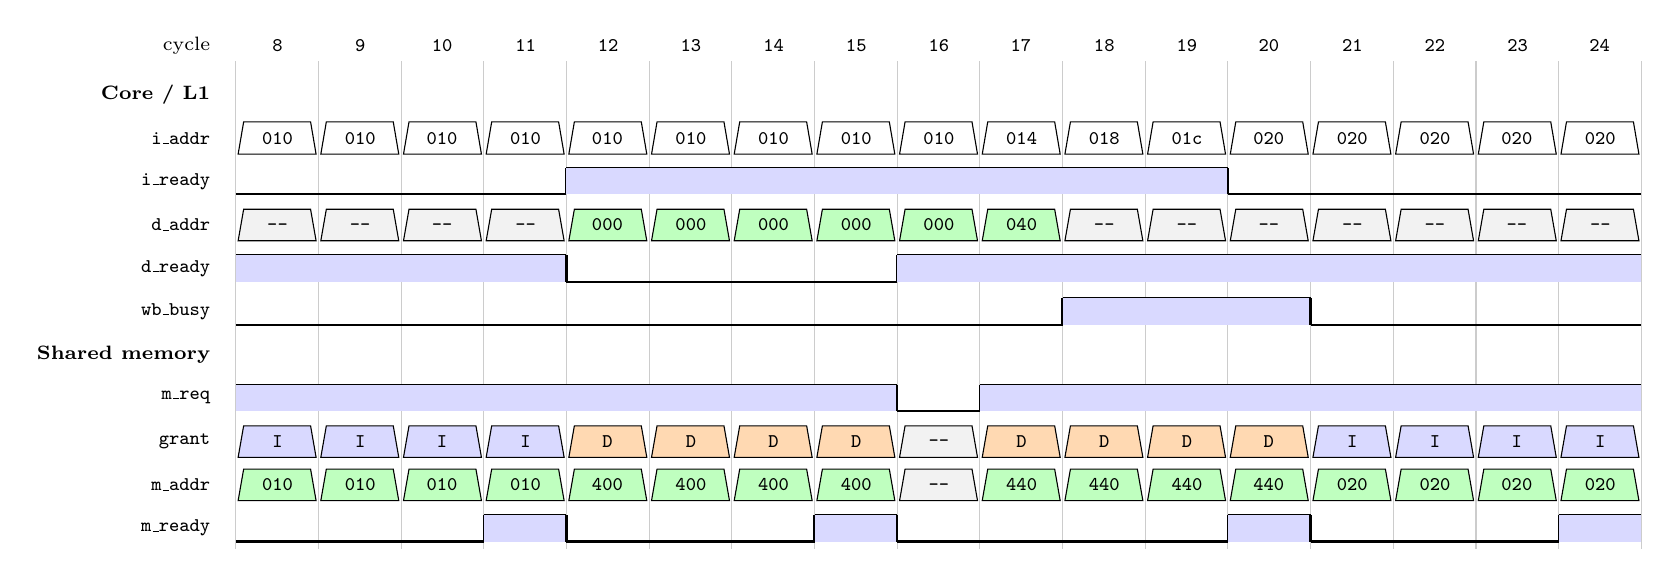
\begin{tikzpicture}[font=\scriptsize\ttfamily, x=1cm, y=1cm]
\node at (0.53,0.35) {8};
\node at (1.58,0.35) {9};
\node at (2.62,0.35) {10};
\node at (3.68,0.35) {11};
\node at (4.73,0.35) {12};
\node at (5.78,0.35) {13};
\node at (6.83,0.35) {14};
\node at (7.88,0.35) {15};
\node at (8.93,0.35) {16};
\node at (9.97,0.35) {17};
\node at (11.03,0.35) {18};
\node at (12.08,0.35) {19};
\node at (13.12,0.35) {20};
\node at (14.18,0.35) {21};
\node at (15.23,0.35) {22};
\node at (16.28,0.35) {23};
\node at (17.32,0.35) {24};
\node[anchor=east] at (-0.2,0.35) {\normalfont cycle};
\draw[gray!40] (0.00,0.15) -- (0.00,-6.05);
\draw[gray!40] (1.05,0.15) -- (1.05,-6.05);
\draw[gray!40] (2.10,0.15) -- (2.10,-6.05);
\draw[gray!40] (3.15,0.15) -- (3.15,-6.05);
\draw[gray!40] (4.20,0.15) -- (4.20,-6.05);
\draw[gray!40] (5.25,0.15) -- (5.25,-6.05);
\draw[gray!40] (6.30,0.15) -- (6.30,-6.05);
\draw[gray!40] (7.35,0.15) -- (7.35,-6.05);
\draw[gray!40] (8.40,0.15) -- (8.40,-6.05);
\draw[gray!40] (9.45,0.15) -- (9.45,-6.05);
\draw[gray!40] (10.50,0.15) -- (10.50,-6.05);
\draw[gray!40] (11.55,0.15) -- (11.55,-6.05);
\draw[gray!40] (12.60,0.15) -- (12.60,-6.05);
\draw[gray!40] (13.65,0.15) -- (13.65,-6.05);
\draw[gray!40] (14.70,0.15) -- (14.70,-6.05);
\draw[gray!40] (15.75,0.15) -- (15.75,-6.05);
\draw[gray!40] (16.80,0.15) -- (16.80,-6.05);
\draw[gray!40] (17.85,0.15) -- (17.85,-6.05);
\node[anchor=east,font=\normalfont\bfseries\scriptsize] at (-0.2,-0.28) {Core / L1};
\node[anchor=east] at (-0.2,-0.83) {i\_addr};
\draw[fill=white] (0.03,-1.03) -- (0.10,-0.62) -- (0.95,-0.62) -- (1.02,-1.03) -- cycle;
\node at (0.53,-0.83) {010};
\draw[fill=white] (1.08,-1.03) -- (1.15,-0.62) -- (2.00,-0.62) -- (2.07,-1.03) -- cycle;
\node at (1.58,-0.83) {010};
\draw[fill=white] (2.13,-1.03) -- (2.20,-0.62) -- (3.05,-0.62) -- (3.12,-1.03) -- cycle;
\node at (2.62,-0.83) {010};
\draw[fill=white] (3.18,-1.03) -- (3.25,-0.62) -- (4.10,-0.62) -- (4.17,-1.03) -- cycle;
\node at (3.68,-0.83) {010};
\draw[fill=white] (4.23,-1.03) -- (4.30,-0.62) -- (5.15,-0.62) -- (5.22,-1.03) -- cycle;
\node at (4.72,-0.83) {010};
\draw[fill=white] (5.28,-1.03) -- (5.35,-0.62) -- (6.20,-0.62) -- (6.27,-1.03) -- cycle;
\node at (5.78,-0.83) {010};
\draw[fill=white] (6.33,-1.03) -- (6.40,-0.62) -- (7.25,-0.62) -- (7.32,-1.03) -- cycle;
\node at (6.83,-0.83) {010};
\draw[fill=white] (7.38,-1.03) -- (7.45,-0.62) -- (8.30,-0.62) -- (8.37,-1.03) -- cycle;
\node at (7.88,-0.83) {010};
\draw[fill=white] (8.43,-1.03) -- (8.50,-0.62) -- (9.35,-0.62) -- (9.42,-1.03) -- cycle;
\node at (8.93,-0.83) {010};
\draw[fill=white] (9.48,-1.03) -- (9.55,-0.62) -- (10.40,-0.62) -- (10.47,-1.03) -- cycle;
\node at (9.98,-0.83) {014};
\draw[fill=white] (10.53,-1.03) -- (10.60,-0.62) -- (11.45,-0.62) -- (11.52,-1.03) -- cycle;
\node at (11.03,-0.83) {018};
\draw[fill=white] (11.58,-1.03) -- (11.65,-0.62) -- (12.50,-0.62) -- (12.57,-1.03) -- cycle;
\node at (12.08,-0.83) {01c};
\draw[fill=white] (12.63,-1.03) -- (12.70,-0.62) -- (13.55,-0.62) -- (13.62,-1.03) -- cycle;
\node at (13.12,-0.83) {020};
\draw[fill=white] (13.68,-1.03) -- (13.75,-0.62) -- (14.60,-0.62) -- (14.67,-1.03) -- cycle;
\node at (14.18,-0.83) {020};
\draw[fill=white] (14.73,-1.03) -- (14.80,-0.62) -- (15.65,-0.62) -- (15.72,-1.03) -- cycle;
\node at (15.23,-0.83) {020};
\draw[fill=white] (15.78,-1.03) -- (15.85,-0.62) -- (16.70,-0.62) -- (16.77,-1.03) -- cycle;
\node at (16.27,-0.83) {020};
\draw[fill=white] (16.83,-1.03) -- (16.90,-0.62) -- (17.75,-0.62) -- (17.82,-1.03) -- cycle;
\node at (17.33,-0.83) {020};
\node[anchor=east] at (-0.2,-1.38) {i\_ready};
\draw[thick] (0.00,-1.54) -- (1.05,-1.54);
\draw[thick] (1.05,-1.54) -- (2.10,-1.54);
\draw[thick] (2.10,-1.54) -- (3.15,-1.54);
\draw[thick] (3.15,-1.54) -- (4.20,-1.54);
\draw[thick] (4.20,-1.21) -- (5.25,-1.21);
\draw[thick] (4.20,-1.54) -- (4.20,-1.21);
\fill[blue!15] (4.20,-1.54) rectangle (5.25,-1.21);
\draw[thick] (5.25,-1.21) -- (6.30,-1.21);
\fill[blue!15] (5.25,-1.54) rectangle (6.30,-1.21);
\draw[thick] (6.30,-1.21) -- (7.35,-1.21);
\fill[blue!15] (6.30,-1.54) rectangle (7.35,-1.21);
\draw[thick] (7.35,-1.21) -- (8.40,-1.21);
\fill[blue!15] (7.35,-1.54) rectangle (8.40,-1.21);
\draw[thick] (8.40,-1.21) -- (9.45,-1.21);
\fill[blue!15] (8.40,-1.54) rectangle (9.45,-1.21);
\draw[thick] (9.45,-1.21) -- (10.50,-1.21);
\fill[blue!15] (9.45,-1.54) rectangle (10.50,-1.21);
\draw[thick] (10.50,-1.21) -- (11.55,-1.21);
\fill[blue!15] (10.50,-1.54) rectangle (11.55,-1.21);
\draw[thick] (11.55,-1.21) -- (12.60,-1.21);
\fill[blue!15] (11.55,-1.54) rectangle (12.60,-1.21);
\draw[thick] (12.60,-1.54) -- (13.65,-1.54);
\draw[thick] (12.60,-1.54) -- (12.60,-1.21);
\draw[thick] (13.65,-1.54) -- (14.70,-1.54);
\draw[thick] (14.70,-1.54) -- (15.75,-1.54);
\draw[thick] (15.75,-1.54) -- (16.80,-1.54);
\draw[thick] (16.80,-1.54) -- (17.85,-1.54);
\node[anchor=east] at (-0.2,-1.93) {d\_addr};
\draw[fill=gray!10] (0.03,-2.13) -- (0.10,-1.73) -- (0.95,-1.73) -- (1.02,-2.13) -- cycle;
\node at (0.53,-1.93) {--};
\draw[fill=gray!10] (1.08,-2.13) -- (1.15,-1.73) -- (2.00,-1.73) -- (2.07,-2.13) -- cycle;
\node at (1.58,-1.93) {--};
\draw[fill=gray!10] (2.13,-2.13) -- (2.20,-1.73) -- (3.05,-1.73) -- (3.12,-2.13) -- cycle;
\node at (2.62,-1.93) {--};
\draw[fill=gray!10] (3.18,-2.13) -- (3.25,-1.73) -- (4.10,-1.73) -- (4.17,-2.13) -- cycle;
\node at (3.68,-1.93) {--};
\draw[fill=green!25] (4.23,-2.13) -- (4.30,-1.73) -- (5.15,-1.73) -- (5.22,-2.13) -- cycle;
\node at (4.72,-1.93) {000};
\draw[fill=green!25] (5.28,-2.13) -- (5.35,-1.73) -- (6.20,-1.73) -- (6.27,-2.13) -- cycle;
\node at (5.78,-1.93) {000};
\draw[fill=green!25] (6.33,-2.13) -- (6.40,-1.73) -- (7.25,-1.73) -- (7.32,-2.13) -- cycle;
\node at (6.83,-1.93) {000};
\draw[fill=green!25] (7.38,-2.13) -- (7.45,-1.73) -- (8.30,-1.73) -- (8.37,-2.13) -- cycle;
\node at (7.88,-1.93) {000};
\draw[fill=green!25] (8.43,-2.13) -- (8.50,-1.73) -- (9.35,-1.73) -- (9.42,-2.13) -- cycle;
\node at (8.93,-1.93) {000};
\draw[fill=green!25] (9.48,-2.13) -- (9.55,-1.73) -- (10.40,-1.73) -- (10.47,-2.13) -- cycle;
\node at (9.98,-1.93) {040};
\draw[fill=gray!10] (10.53,-2.13) -- (10.60,-1.73) -- (11.45,-1.73) -- (11.52,-2.13) -- cycle;
\node at (11.03,-1.93) {--};
\draw[fill=gray!10] (11.58,-2.13) -- (11.65,-1.73) -- (12.50,-1.73) -- (12.57,-2.13) -- cycle;
\node at (12.08,-1.93) {--};
\draw[fill=gray!10] (12.63,-2.13) -- (12.70,-1.73) -- (13.55,-1.73) -- (13.62,-2.13) -- cycle;
\node at (13.12,-1.93) {--};
\draw[fill=gray!10] (13.68,-2.13) -- (13.75,-1.73) -- (14.60,-1.73) -- (14.67,-2.13) -- cycle;
\node at (14.18,-1.93) {--};
\draw[fill=gray!10] (14.73,-2.13) -- (14.80,-1.73) -- (15.65,-1.73) -- (15.72,-2.13) -- cycle;
\node at (15.23,-1.93) {--};
\draw[fill=gray!10] (15.78,-2.13) -- (15.85,-1.73) -- (16.70,-1.73) -- (16.77,-2.13) -- cycle;
\node at (16.27,-1.93) {--};
\draw[fill=gray!10] (16.83,-2.13) -- (16.90,-1.73) -- (17.75,-1.73) -- (17.82,-2.13) -- cycle;
\node at (17.33,-1.93) {--};
\node[anchor=east] at (-0.2,-2.48) {d\_ready};
\draw[thick] (0.00,-2.31) -- (1.05,-2.31);
\fill[blue!15] (0.00,-2.65) rectangle (1.05,-2.31);
\draw[thick] (1.05,-2.31) -- (2.10,-2.31);
\fill[blue!15] (1.05,-2.65) rectangle (2.10,-2.31);
\draw[thick] (2.10,-2.31) -- (3.15,-2.31);
\fill[blue!15] (2.10,-2.65) rectangle (3.15,-2.31);
\draw[thick] (3.15,-2.31) -- (4.20,-2.31);
\fill[blue!15] (3.15,-2.65) rectangle (4.20,-2.31);
\draw[thick] (4.20,-2.65) -- (5.25,-2.65);
\draw[thick] (4.20,-2.65) -- (4.20,-2.31);
\draw[thick] (5.25,-2.65) -- (6.30,-2.65);
\draw[thick] (6.30,-2.65) -- (7.35,-2.65);
\draw[thick] (7.35,-2.65) -- (8.40,-2.65);
\draw[thick] (8.40,-2.31) -- (9.45,-2.31);
\draw[thick] (8.40,-2.65) -- (8.40,-2.31);
\fill[blue!15] (8.40,-2.65) rectangle (9.45,-2.31);
\draw[thick] (9.45,-2.31) -- (10.50,-2.31);
\fill[blue!15] (9.45,-2.65) rectangle (10.50,-2.31);
\draw[thick] (10.50,-2.31) -- (11.55,-2.31);
\fill[blue!15] (10.50,-2.65) rectangle (11.55,-2.31);
\draw[thick] (11.55,-2.31) -- (12.60,-2.31);
\fill[blue!15] (11.55,-2.65) rectangle (12.60,-2.31);
\draw[thick] (12.60,-2.31) -- (13.65,-2.31);
\fill[blue!15] (12.60,-2.65) rectangle (13.65,-2.31);
\draw[thick] (13.65,-2.31) -- (14.70,-2.31);
\fill[blue!15] (13.65,-2.65) rectangle (14.70,-2.31);
\draw[thick] (14.70,-2.31) -- (15.75,-2.31);
\fill[blue!15] (14.70,-2.65) rectangle (15.75,-2.31);
\draw[thick] (15.75,-2.31) -- (16.80,-2.31);
\fill[blue!15] (15.75,-2.65) rectangle (16.80,-2.31);
\draw[thick] (16.80,-2.31) -- (17.85,-2.31);
\fill[blue!15] (16.80,-2.65) rectangle (17.85,-2.31);
\node[anchor=east] at (-0.2,-3.03) {wb\_busy};
\draw[thick] (0.00,-3.20) -- (1.05,-3.20);
\draw[thick] (1.05,-3.20) -- (2.10,-3.20);
\draw[thick] (2.10,-3.20) -- (3.15,-3.20);
\draw[thick] (3.15,-3.20) -- (4.20,-3.20);
\draw[thick] (4.20,-3.20) -- (5.25,-3.20);
\draw[thick] (5.25,-3.20) -- (6.30,-3.20);
\draw[thick] (6.30,-3.20) -- (7.35,-3.20);
\draw[thick] (7.35,-3.20) -- (8.40,-3.20);
\draw[thick] (8.40,-3.20) -- (9.45,-3.20);
\draw[thick] (9.45,-3.20) -- (10.50,-3.20);
\draw[thick] (10.50,-2.86) -- (11.55,-2.86);
\draw[thick] (10.50,-3.20) -- (10.50,-2.86);
\fill[blue!15] (10.50,-3.20) rectangle (11.55,-2.86);
\draw[thick] (11.55,-2.86) -- (12.60,-2.86);
\fill[blue!15] (11.55,-3.20) rectangle (12.60,-2.86);
\draw[thick] (12.60,-2.86) -- (13.65,-2.86);
\fill[blue!15] (12.60,-3.20) rectangle (13.65,-2.86);
\draw[thick] (13.65,-3.20) -- (14.70,-3.20);
\draw[thick] (13.65,-3.20) -- (13.65,-2.86);
\draw[thick] (14.70,-3.20) -- (15.75,-3.20);
\draw[thick] (15.75,-3.20) -- (16.80,-3.20);
\draw[thick] (16.80,-3.20) -- (17.85,-3.20);
\node[anchor=east,font=\normalfont\bfseries\scriptsize] at (-0.2,-3.58) {Shared memory};
\node[anchor=east] at (-0.2,-4.12) {m\_req};
\draw[thick] (0.00,-3.96) -- (1.05,-3.96);
\fill[blue!15] (0.00,-4.29) rectangle (1.05,-3.96);
\draw[thick] (1.05,-3.96) -- (2.10,-3.96);
\fill[blue!15] (1.05,-4.29) rectangle (2.10,-3.96);
\draw[thick] (2.10,-3.96) -- (3.15,-3.96);
\fill[blue!15] (2.10,-4.29) rectangle (3.15,-3.96);
\draw[thick] (3.15,-3.96) -- (4.20,-3.96);
\fill[blue!15] (3.15,-4.29) rectangle (4.20,-3.96);
\draw[thick] (4.20,-3.96) -- (5.25,-3.96);
\fill[blue!15] (4.20,-4.29) rectangle (5.25,-3.96);
\draw[thick] (5.25,-3.96) -- (6.30,-3.96);
\fill[blue!15] (5.25,-4.29) rectangle (6.30,-3.96);
\draw[thick] (6.30,-3.96) -- (7.35,-3.96);
\fill[blue!15] (6.30,-4.29) rectangle (7.35,-3.96);
\draw[thick] (7.35,-3.96) -- (8.40,-3.96);
\fill[blue!15] (7.35,-4.29) rectangle (8.40,-3.96);
\draw[thick] (8.40,-4.29) -- (9.45,-4.29);
\draw[thick] (8.40,-4.29) -- (8.40,-3.96);
\draw[thick] (9.45,-3.96) -- (10.50,-3.96);
\draw[thick] (9.45,-4.29) -- (9.45,-3.96);
\fill[blue!15] (9.45,-4.29) rectangle (10.50,-3.96);
\draw[thick] (10.50,-3.96) -- (11.55,-3.96);
\fill[blue!15] (10.50,-4.29) rectangle (11.55,-3.96);
\draw[thick] (11.55,-3.96) -- (12.60,-3.96);
\fill[blue!15] (11.55,-4.29) rectangle (12.60,-3.96);
\draw[thick] (12.60,-3.96) -- (13.65,-3.96);
\fill[blue!15] (12.60,-4.29) rectangle (13.65,-3.96);
\draw[thick] (13.65,-3.96) -- (14.70,-3.96);
\fill[blue!15] (13.65,-4.29) rectangle (14.70,-3.96);
\draw[thick] (14.70,-3.96) -- (15.75,-3.96);
\fill[blue!15] (14.70,-4.29) rectangle (15.75,-3.96);
\draw[thick] (15.75,-3.96) -- (16.80,-3.96);
\fill[blue!15] (15.75,-4.29) rectangle (16.80,-3.96);
\draw[thick] (16.80,-3.96) -- (17.85,-3.96);
\fill[blue!15] (16.80,-4.29) rectangle (17.85,-3.96);
\node[anchor=east] at (-0.2,-4.68) {grant};
\draw[fill=blue!15] (0.03,-4.88) -- (0.10,-4.48) -- (0.95,-4.48) -- (1.02,-4.88) -- cycle;
\node at (0.53,-4.68) {I};
\draw[fill=blue!15] (1.08,-4.88) -- (1.15,-4.48) -- (2.00,-4.48) -- (2.07,-4.88) -- cycle;
\node at (1.58,-4.68) {I};
\draw[fill=blue!15] (2.13,-4.88) -- (2.20,-4.48) -- (3.05,-4.48) -- (3.12,-4.88) -- cycle;
\node at (2.62,-4.68) {I};
\draw[fill=blue!15] (3.18,-4.88) -- (3.25,-4.48) -- (4.10,-4.48) -- (4.17,-4.88) -- cycle;
\node at (3.68,-4.68) {I};
\draw[fill=orange!30] (4.23,-4.88) -- (4.30,-4.48) -- (5.15,-4.48) -- (5.22,-4.88) -- cycle;
\node at (4.72,-4.68) {D};
\draw[fill=orange!30] (5.28,-4.88) -- (5.35,-4.48) -- (6.20,-4.48) -- (6.27,-4.88) -- cycle;
\node at (5.78,-4.68) {D};
\draw[fill=orange!30] (6.33,-4.88) -- (6.40,-4.48) -- (7.25,-4.48) -- (7.32,-4.88) -- cycle;
\node at (6.83,-4.68) {D};
\draw[fill=orange!30] (7.38,-4.88) -- (7.45,-4.48) -- (8.30,-4.48) -- (8.37,-4.88) -- cycle;
\node at (7.88,-4.68) {D};
\draw[fill=gray!10] (8.43,-4.88) -- (8.50,-4.48) -- (9.35,-4.48) -- (9.42,-4.88) -- cycle;
\node at (8.93,-4.68) {--};
\draw[fill=orange!30] (9.48,-4.88) -- (9.55,-4.48) -- (10.40,-4.48) -- (10.47,-4.88) -- cycle;
\node at (9.98,-4.68) {D};
\draw[fill=orange!30] (10.53,-4.88) -- (10.60,-4.48) -- (11.45,-4.48) -- (11.52,-4.88) -- cycle;
\node at (11.03,-4.68) {D};
\draw[fill=orange!30] (11.58,-4.88) -- (11.65,-4.48) -- (12.50,-4.48) -- (12.57,-4.88) -- cycle;
\node at (12.08,-4.68) {D};
\draw[fill=orange!30] (12.63,-4.88) -- (12.70,-4.48) -- (13.55,-4.48) -- (13.62,-4.88) -- cycle;
\node at (13.12,-4.68) {D};
\draw[fill=blue!15] (13.68,-4.88) -- (13.75,-4.48) -- (14.60,-4.48) -- (14.67,-4.88) -- cycle;
\node at (14.18,-4.68) {I};
\draw[fill=blue!15] (14.73,-4.88) -- (14.80,-4.48) -- (15.65,-4.48) -- (15.72,-4.88) -- cycle;
\node at (15.23,-4.68) {I};
\draw[fill=blue!15] (15.78,-4.88) -- (15.85,-4.48) -- (16.70,-4.48) -- (16.77,-4.88) -- cycle;
\node at (16.27,-4.68) {I};
\draw[fill=blue!15] (16.83,-4.88) -- (16.90,-4.48) -- (17.75,-4.48) -- (17.82,-4.88) -- cycle;
\node at (17.33,-4.68) {I};
\node[anchor=east] at (-0.2,-5.23) {m\_addr};
\draw[fill=green!25] (0.03,-5.43) -- (0.10,-5.03) -- (0.95,-5.03) -- (1.02,-5.43) -- cycle;
\node at (0.53,-5.23) {010};
\draw[fill=green!25] (1.08,-5.43) -- (1.15,-5.03) -- (2.00,-5.03) -- (2.07,-5.43) -- cycle;
\node at (1.58,-5.23) {010};
\draw[fill=green!25] (2.13,-5.43) -- (2.20,-5.03) -- (3.05,-5.03) -- (3.12,-5.43) -- cycle;
\node at (2.62,-5.23) {010};
\draw[fill=green!25] (3.18,-5.43) -- (3.25,-5.03) -- (4.10,-5.03) -- (4.17,-5.43) -- cycle;
\node at (3.68,-5.23) {010};
\draw[fill=green!25] (4.23,-5.43) -- (4.30,-5.03) -- (5.15,-5.03) -- (5.22,-5.43) -- cycle;
\node at (4.72,-5.23) {400};
\draw[fill=green!25] (5.28,-5.43) -- (5.35,-5.03) -- (6.20,-5.03) -- (6.27,-5.43) -- cycle;
\node at (5.78,-5.23) {400};
\draw[fill=green!25] (6.33,-5.43) -- (6.40,-5.03) -- (7.25,-5.03) -- (7.32,-5.43) -- cycle;
\node at (6.83,-5.23) {400};
\draw[fill=green!25] (7.38,-5.43) -- (7.45,-5.03) -- (8.30,-5.03) -- (8.37,-5.43) -- cycle;
\node at (7.88,-5.23) {400};
\draw[fill=gray!10] (8.43,-5.43) -- (8.50,-5.03) -- (9.35,-5.03) -- (9.42,-5.43) -- cycle;
\node at (8.93,-5.23) {--};
\draw[fill=green!25] (9.48,-5.43) -- (9.55,-5.03) -- (10.40,-5.03) -- (10.47,-5.43) -- cycle;
\node at (9.98,-5.23) {440};
\draw[fill=green!25] (10.53,-5.43) -- (10.60,-5.03) -- (11.45,-5.03) -- (11.52,-5.43) -- cycle;
\node at (11.03,-5.23) {440};
\draw[fill=green!25] (11.58,-5.43) -- (11.65,-5.03) -- (12.50,-5.03) -- (12.57,-5.43) -- cycle;
\node at (12.08,-5.23) {440};
\draw[fill=green!25] (12.63,-5.43) -- (12.70,-5.03) -- (13.55,-5.03) -- (13.62,-5.43) -- cycle;
\node at (13.12,-5.23) {440};
\draw[fill=green!25] (13.68,-5.43) -- (13.75,-5.03) -- (14.60,-5.03) -- (14.67,-5.43) -- cycle;
\node at (14.18,-5.23) {020};
\draw[fill=green!25] (14.73,-5.43) -- (14.80,-5.03) -- (15.65,-5.03) -- (15.72,-5.43) -- cycle;
\node at (15.23,-5.23) {020};
\draw[fill=green!25] (15.78,-5.43) -- (15.85,-5.03) -- (16.70,-5.03) -- (16.77,-5.43) -- cycle;
\node at (16.27,-5.23) {020};
\draw[fill=green!25] (16.83,-5.43) -- (16.90,-5.03) -- (17.75,-5.03) -- (17.82,-5.43) -- cycle;
\node at (17.33,-5.23) {020};
\node[anchor=east] at (-0.2,-5.78) {m\_ready};
\draw[thick] (0.00,-5.95) -- (1.05,-5.95);
\draw[thick] (1.05,-5.95) -- (2.10,-5.95);
\draw[thick] (2.10,-5.95) -- (3.15,-5.95);
\draw[thick] (3.15,-5.61) -- (4.20,-5.61);
\draw[thick] (3.15,-5.95) -- (3.15,-5.61);
\fill[blue!15] (3.15,-5.95) rectangle (4.20,-5.61);
\draw[thick] (4.20,-5.95) -- (5.25,-5.95);
\draw[thick] (4.20,-5.95) -- (4.20,-5.61);
\draw[thick] (5.25,-5.95) -- (6.30,-5.95);
\draw[thick] (6.30,-5.95) -- (7.35,-5.95);
\draw[thick] (7.35,-5.61) -- (8.40,-5.61);
\draw[thick] (7.35,-5.95) -- (7.35,-5.61);
\fill[blue!15] (7.35,-5.95) rectangle (8.40,-5.61);
\draw[thick] (8.40,-5.95) -- (9.45,-5.95);
\draw[thick] (8.40,-5.95) -- (8.40,-5.61);
\draw[thick] (9.45,-5.95) -- (10.50,-5.95);
\draw[thick] (10.50,-5.95) -- (11.55,-5.95);
\draw[thick] (11.55,-5.95) -- (12.60,-5.95);
\draw[thick] (12.60,-5.61) -- (13.65,-5.61);
\draw[thick] (12.60,-5.95) -- (12.60,-5.61);
\fill[blue!15] (12.60,-5.95) rectangle (13.65,-5.61);
\draw[thick] (13.65,-5.95) -- (14.70,-5.95);
\draw[thick] (13.65,-5.95) -- (13.65,-5.61);
\draw[thick] (14.70,-5.95) -- (15.75,-5.95);
\draw[thick] (15.75,-5.95) -- (16.80,-5.95);
\draw[thick] (16.80,-5.61) -- (17.85,-5.61);
\draw[thick] (16.80,-5.95) -- (16.80,-5.61);
\fill[blue!15] (16.80,-5.95) rectangle (17.85,-5.61);
\end{tikzpicture}
}
  \caption{Phase II, \sig{memcopy} on the modified Harvard system ($N=8$, $L=4$, write buffer
  on), cycles 8--24, generated from the simulation trace by \sig{tools/vcd2tikz.py}. Instruction
  miss, data miss, buffered store overlapping execution, and an instruction miss that waits for
  the store to drain (no pre-emption).}
  \label{fig:wave2}
\end{figure*}

\subsection{CPI vs memory latency}
Fig.~\ref{fig:cpi} shows the suite CPI (total cycles divided by total instructions over all
eight programs) as the memory latency grows, with $N=8$ lines per split cache and the write
buffer on. The ideal Harvard system stays at 1.00 and the Phase~I baseline at 1.24. Without a
cache, every fetch and every data access pays the full latency, so the CPI grows almost
linearly, reaching 9.88 at $L=8$ and 19.7 at $L=16$. The caches hide most of this. At $L=8$ the
modified Harvard system reaches 1.69 and the unified system 2.72, and both grow far more slowly
than the no-cache system. At $L=1$ the caches \emph{cost} cycles. No-cache at $L=1$ is the
Phase~I baseline (1.24), but the unified system needs 1.39, because every miss still costs a
cycle and code and data evict each other. Caches pay off as soon as $L\ge2$.

\begin{figure}[t]
  \centering
  \begin{tikzpicture}
    \begin{axis}[width=\columnwidth, height=5.4cm, xmode=log, log basis x=2, ymode=log,
        xlabel={memory latency $L$ (cycles)}, ylabel={suite CPI},
        xtick={1,2,4,8,16}, xticklabels={1,2,4,8,16},
        ytick={1,1.5,2,3,5,10,20}, yticklabels={1,1.5,2,3,5,10,20},
        legend style={font=\scriptsize, cells={anchor=west}, at={(0.5,-0.32)}, anchor=north,
          legend columns=2},
        grid=major, grid style={gray!25}, tick label style={font=\scriptsize}]
      \addplot[thick, black, mark=*, mark size=1.4pt] table[x=L, y=nocache] {data/cpi_latency.dat};
      \addlegendentry{no cache (single bus)}
      \addplot[thick, red!70!black, mark=square*, mark size=1.4pt] table[x=L, y=unified] {data/cpi_latency.dat};
      \addlegendentry{unified cache, $2N$ lines}
      \addplot[thick, blue!70!black, mark=triangle*, mark size=1.8pt] table[x=L, y=mh] {data/cpi_latency.dat};
      \addlegendentry{modified Harvard, $N{+}N$ lines}
      \addplot[thick, dashed, gray] table[x=L, y=vnideal] {data/cpi_latency.dat};
      \addlegendentry{Phase I baseline (ideal)}
      \addplot[thick, dotted, black] table[x=L, y=ideal] {data/cpi_latency.dat};
      \addlegendentry{ideal Harvard}
    \end{axis}
  \end{tikzpicture}
  \caption{Suite CPI vs memory latency ($N=8$, 4-word lines, write buffer on), plotted from
  \sig{sweep.csv}. Both axes are logarithmic.}
  \label{fig:cpi}
\end{figure}

\subsection{Write-buffer ablation}
Table~\ref{tab:wbuf} compares the cycle counts with the write buffer off and on at $L=8$,
$N=8$. For the store-heavy programs the buffer removes 22--26\% of the cycles of the modified
Harvard system. Over the whole suite it removes 15.1\% (5618 to 4768 cycles), and 10.1\% for the
unified system (8547 to 7688). The gain is smaller than the stores' share of the time, for the
three reasons Skadron and Clark give \cite{skadron1997}:
\begin{itemize}
  \item a one-entry buffer is often still busy when the next store arrives: \sig{bubble\_sort}
        writes its swaps in pairs and spends 429 cycles waiting for the buffer;
  \item a read miss must wait until the buffer has drained;
  \item a draining store blocks the next instruction refill, which shows up as arbiter
        conflicts (12 cycles in \sig{bubble\_sort}, 23 in \sig{subroutine}).
\end{itemize}
Without a cache the buffer gains nothing (27947 cycles both ways): every following fetch needs
the same memory port anyway, so it simply waits for the drain instead of for the store.

\begin{table}[t]
  \caption{Write-buffer ablation, $L=8$, $N=8$: cycles without / with the buffer}
  \label{tab:wbuf}
  \centering
  \setlength{\tabcolsep}{3pt}
  \begin{tabular}{@{}lrrrrrr@{}}
    \toprule
    & & \multicolumn{3}{c}{Modified Harvard} & \multicolumn{2}{c}{Unified} \\
    \cmidrule(lr){3-5}\cmidrule(lr){6-7}
    Program & Stores & off & on & gain & off & on \\
    \midrule
    \tabinput{data/tab_wbuf.tex}
    \bottomrule
  \end{tabular}
\end{table}

% Owner: Ankit (Member 3)
\subsection{Split vs unified caches}
\label{sec:split}
Table~\ref{tab:split} compares the modified Harvard system ($8+8$ lines) with the unified
system (16 lines) at $L=8$. The split design is faster on seven of the eight programs, by up to
2.68$\times$. Two separate effects cause this.

\textbf{Single port.} Even with perfect caches, the single-bus core fetches and accesses data in
different cycles, so its CPI cannot fall below $1+f_{\text{LS}}$: 1.41 for \sig{bubble\_sort},
for example. The split design can overlap a hit in each cache in the same cycle. This is the
Phase~I result, still present one level up.

\textbf{Code/data conflict misses.} The unified cache misses far more often: 262 times on
\sig{bubble\_sort}, against 11 for the split pair. Code starts at physical \texttt{0x000} and
data at \texttt{0x400}. Every unified size we test (up to 64 lines, 1\,KB) divides
\texttt{0x400}, so code word $k$ and data word $k$ always map to the same line. Both loops of
\sig{bubble\_sort} sit in code lines 0--3, and its 16-word array occupies the same four cache
lines, so code and data evict each other on every iteration. These are conflict misses in the sense of Hill and Smith
\cite{hill1989}. A larger direct-mapped cache cannot remove them, which is why the unified miss
count stays flat in Fig.~\ref{fig:size}.

\begin{table}[t]
  \caption{Split ($8+8$ lines) vs unified (16 lines), $L=8$, write buffer on}
  \label{tab:split}
  \centering
  \setlength{\tabcolsep}{2.6pt}
  \begin{tabular}{@{}lrrrrrrr@{}}
    \toprule
    & \multicolumn{2}{c}{Split misses} & \multicolumn{2}{c}{Unified misses} &
      \multicolumn{2}{c}{CPI} & Unified/ \\
    \cmidrule(lr){2-3}\cmidrule(lr){4-5}\cmidrule(lr){6-7}
    Program & I & D & fetch & data & split & unified & split \\
    \midrule
    \tabinput{data/tab_split.tex}
    \bottomrule
  \end{tabular}
\end{table}

\textbf{Where unified wins.} The unified cache wins when its shared capacity matters more than
these two penalties:
\begin{itemize}
  \item \sig{subroutine} has a 59-word (15-line) code footprint and very little data. An 8-line
        I-cache cannot hold it (75 I-misses), while a 16-line unified cache holds most of it
        (55 misses in all). At $N=8$ the unified system is therefore faster (CPI 1.53 vs 1.71,
        a ratio of 0.89$\times$ in Table~\ref{tab:split}), even though it pays the single-port
        penalty.
  \item With one line per split cache, the unified pair of lines wins for the whole suite
        (1019 vs 1168 misses, CPI 4.47 vs 4.70). The 2-line cache can keep a loop's code line
        and its data line at the same time, while a one-line I-cache thrashes on any loop that
        crosses a line boundary.
\end{itemize}
Smith predicts exactly this behaviour \cite{smith1982}: a unified cache adapts to the mix of
code and data, while a split cache wastes the capacity of the side that does not need it.

\begin{figure}[t]
  \centering
  \begin{tikzpicture}
    \begin{axis}[width=\columnwidth, height=5.4cm, xmode=log, log basis x=2, ymode=log,
        xlabel={lines per split cache $N$ (unified: $2N$)}, ylabel={total misses, 8 programs},
        xtick={1,2,4,8,16,32}, xticklabels={1,2,4,8,16,32},
        legend style={font=\scriptsize, cells={anchor=west}, at={(0.5,-0.32)}, anchor=north},
        grid=major, grid style={gray!25}, tick label style={font=\scriptsize}]
      \addplot[thick, blue!70!black, mark=triangle*, mark size=1.8pt] table[x=N, y=split] {data/size_suite.dat};
      \addlegendentry{split I + D (any placement)}
      \addplot[thick, red!70!black, mark=square*, mark size=1.4pt] table[x=N, y=unified] {data/size_suite.dat};
      \addlegendentry{unified, data at \texttt{0x400}}
      \addplot[thick, dashed, red!70!black, mark=o, mark size=1.6pt] table[x=N, y=unified] {data/size_skew_suite.dat};
      \addlegendentry{unified, data at \texttt{0x480}}
    \end{axis}
  \end{tikzpicture}
  \caption{Total misses vs cache size ($L=8$, write buffer on). The unified cache wins at
  $N=1$. With the Phase~I memory map, code and data alias, and a larger unified cache stops
  helping. Moving the data by half a 16-line cache removes most of that aliasing.}
  \label{fig:size}
\end{figure}

\textbf{Placement sensitivity.} To separate the aliasing effect from the organisation itself,
the sweep repeats the $L=8$ runs with the data image moved to physical \texttt{0x480}
(Fig.~\ref{fig:size}, dashed). The split miss counts do not change, which the sweep checks: the
D-cache sees only data, and the shift is a whole number of lines. The unified cache improves
dramatically. At $N=8$ it misses 165 times instead of 438, against 156 for the split pair, and
\sig{bubble\_sort} drops from 262 misses to 11. The suite CPI falls from 2.72 to 1.87, which is
still above the split design's 1.69 because of the single-port penalty. The unified cache is
therefore not inherently much worse than the split pair; most of its deficit in
Table~\ref{tab:split} is the code/data placement. A real system would use a set-associative
cache, or link data at an address that is not a multiple of the cache size.

\subsection{Hardware cost and timing}
\label{sec:area}
Table~\ref{tab:area} gives Yosys \cite{yosys} estimates for a Xilinx 7-series device
(\texttt{synth\_xilinx}, version 0.71). In the cached designs the shared memory is a black box, because it
stands for block RAM or external memory and is the same in every design. The ideal Harvard
system includes the separately synthesised 256-word ROM, as in Phase~I, so the tool cannot
hard-wire one program into the decoder. The modified Harvard system with two 8-line caches
needs about as many LUTs as the single-bus system with no cache, and fewer than the single-bus
system with a 16-line unified cache. Its I-cache has no write path, and the single-bus core needs
its FSM, latched instruction and address multiplexers. In every cached design, 192 of the
roughly 470 flip-flops are the six 32-bit event counters, which exist only for measurement.
Compared with Phase~I (654 and 1084 total LUTs), the extended instruction set, mainly the barrel
shifter and the jump logic, increases the ideal Harvard and baseline designs by 69\% and 29\%.

\begin{table}[t]
  \caption{Synthesis estimate, Yosys \texttt{synth\_xilinx -family xc7}}
  \label{tab:area}
  \centering
  \footnotesize
  \setlength{\tabcolsep}{2.4pt}
  \begin{tabular}{@{}lrrrr@{}}
    \toprule
    Design & Logic & LUT- & Total & FFs \\
           & LUTs  & RAM  & LUTs  &     \\
    \midrule
    \tabinput{data/area.tex}
    \bottomrule
  \end{tabular}
\end{table}

\textbf{Combinational loops.} The modified Harvard design synthesises with no
``logic loop'' warning. To check that the timing rules are what keeps it loop-free,
\sig{results/synth2/loop\_demo.sh} synthesises two broken copies. With refill forwarding,
Yosys reports 92 loop warnings through the arbiter's address multiplexer. With the I-cache
request set to \sig{\textasciitilde halt}, it reports one loop through the EBREAK decoder and the
cache's ready output. Both single-bus systems still report the Phase~I loop
$\sig{m\_addr}\rightarrow$ memory/cache $\rightarrow\sig{m\_rdata}$/\sig{m\_ready}
$\rightarrow$ instruction mux $\rightarrow$ ALU $\rightarrow\sig{m\_addr}$. This loop is a false
path: in \textsc{FetchExec} the bus address is the PC, and in \textsc{Mem} the instruction comes
from the latched register, so no real signal can travel all the way round.

\subsection{Limitations}
\begin{itemize}
  \item No clock frequency was measured for Phase~II. The ECP5 place-and-route tools used in
        Phase~I were not available, and Yosys has no timing model for 7-series devices. The
        synthesis numbers are estimates, not post-route utilisation.
  \item The memory is a simple fixed-latency model that returns a whole line per transfer. A
        DRAM would add variable latency and burst transfers, and the memory itself was not
        synthesised.
  \item The caches are direct-mapped and write-through. Associativity, write-back caches,
        deeper write buffers and prefetching are not modelled.
  \item The benchmarks are small (31--947 instructions) and run from cold caches, so
        compulsory misses carry more weight than they would in long programs.
  \item The counters stop at EBREAK, so a store still draining from the write buffer after the
        halt (at most $L$ cycles) is not counted.
\end{itemize}


% Owner: Anshika (Member 2); each member checks their own row and paragraph.
%=====================================================================
\section{Individual Contributions}
%=====================================================================
Each member worked on their own branch and merged into \sig{main} through pull requests. The
repository's commit history shows the split in Table~\ref{tab:contrib}. Phase~I branches were
\sig{m1-memory} to \sig{m4-verification}. The Phase~II branches and the order in which they
were merged are listed in \sig{docs/phase2\_work\_split.md}. Phase~II was carried out by four
members.

\begin{table*}[t]
  \caption{Individual contributions}
  \label{tab:contrib}
  \centering
  \footnotesize
  \begin{tabular}{@{}l>{\raggedright}p{5.6cm}>{\raggedright\arraybackslash}p{8.4cm}@{}}
    \toprule
    Member & Phase I & Phase II \\
    \midrule
    Yashpal   & Harvard memory: \sig{instr\_mem}, \sig{data\_mem}, \sig{addr\_decoder},
                \sig{rw\_ctrl}, \sig{harvard\_mem}
              & Reusable cache (\sig{cache}: direct-mapped, write-through, no-write-allocate,
                write buffer, uncached mode) and shared memory \sig{main\_mem}; report sections
                on caches (Literature Review) and on the cache and memory (Proposed Solution);
                cache figure \\
    Anshika   & Processor and integration: \sig{pc\_reg}, \sig{regfile}, \sig{alu},
                \sig{imm\_gen}, \sig{control}, \sig{cpu\_core}, \sig{harvard\_top}; repository
                and PR merges
              & Instruction-set extension and stall interface of \sig{cpu\_core}; modified
                Harvard top \sig{mh\_top}; timing rules; report frame, abstract, architecture
                section, Phase~II block diagram, conclusion, contributions; README; PR reviews
                and merges \\
    Ankit     & Baseline and metrics: \sig{perf\_counters}, \sig{shared\_mem},
                \sig{cpu\_core\_vn}, \sig{vn\_top}; comparison; Yosys synthesis; ECP5 Fmax
              & Extension and stall interface of \sig{cpu\_core\_vn}; \sig{arbiter},
                \sig{event\_counters}, single-bus top \sig{vnc\_top}; Phase~II synthesis,
                area table and loop demonstration; report sections on architectures, the
                arbiter, Phase~I results, split vs unified, area and limitations \\
    Samriddhi & Verification: assembler, four programs, unit/system/comparison testbenches,
                \sig{Makefile}, waveform tool
              & Assembler extension, golden-model ISS, four new programs, \sig{tb\_cache},
                \sig{tb\_system}, parameter sweep, Phase~II build targets and waveform figure;
                report sections on verification, timing behaviour, CPI vs latency and the
                write buffer \\
    Ayush     & IEEE report and figures, video script and editing, README and documentation
              & --- \\
    \bottomrule
  \end{tabular}
\end{table*}

\textbf{Yashpal} built the Phase~I Harvard memory subsystem. In Phase~II he designed the
reusable cache module and its hit, refill, write-through and write-buffer logic, so that one
module serves as I-cache, D-cache, unified cache and uncached path. He also built the
fixed-latency shared memory with its request/ready handshake.

\textbf{Anshika} built the Phase~I single-cycle processor and set up the repository. In
Phase~II she added the thirteen new instructions and the \sig{i\_ready}/\sig{d\_ready} stall
interface to \sig{cpu\_core}, proved that Phase~I timing was unchanged, integrated the modified
Harvard top, and enforced the timing rules. She also assembled this report and the README and
merged the other members' pull requests.

\textbf{Ankit} built the Phase~I baseline, the counters and the synthesis and Fmax flow. In
Phase~II he extended the single-bus core with the same instructions and an \sig{m\_ready}
stall, and wrote the arbiter, the event counters and the single-bus top for the unified and
no-cache systems. He synthesised every design, explained the logic-loop warnings, and wrote the
split-versus-unified analysis.

\textbf{Samriddhi} built the Phase~I verification flow. In Phase~II she extended the assembler,
wrote the independent instruction-set simulator used as the golden model, the four new
benchmarks, the cache unit test, the five-system testbench and the sweep that cross-checks
every RTL miss count, and generated all plots and the Phase~II waveform from simulation data.

\textbf{Ayush} wrote the Phase~I report and its figures, produced the prototype video and
maintained the Phase~I documentation. He did not take part in Phase~II.

% Owner: Anshika (Member 2)
%=====================================================================
\section{Conclusion and Future Work}
%=====================================================================
Phase~I showed that separate instruction and data paths remove the structural hazard of a
shared port: CPI\,=\,1.00 against $1+f_{\text{LS}}$. Phase~II moved the comparison to a
realistic hierarchy, with one reusable direct-mapped cache, one shared memory of latency $L$,
and an arbiter. The same RTL and the same memory were measured as a modified Harvard system, as
a single bus with a unified cache of equal capacity, and as a single bus with no cache. An
independent golden model predicted every miss count, and 528 system simulations matched it in
all 9888 checks. Phase~I timing was preserved exactly.

The results lead to three conclusions.
\begin{itemize}
  \item Caches are essential as soon as memory is slower than the core. At $L=8$ the suite CPI
        is 9.88 without a cache, 2.72 with a unified cache and 1.69 with split caches.
  \item The split organisation wins mainly because it keeps two accesses per cycle and keeps
        code and data out of each other's way. With our memory map, most unified misses are
        code/data conflict misses: moving the data by half a cache cuts them from 438 to 165.
        The unified cache wins only when the code footprint is larger than the I-cache, or when
        both caches are tiny.
  \item A one-entry write buffer removes 15\% of the cycles of the split design. It is limited by
        back-to-back stores and by drains that delay instruction refills. Without a cache it
        cannot help at all.
\end{itemize}
The modified Harvard design synthesises without combinational loops, because refill data is
never forwarded and the I-cache request comes from a register.

\textbf{Future work.} The next steps are:
\begin{itemize}
  \item set-associative caches and a victim cache \cite{jouppi1990}, to remove the conflict
        misses measured here;
  \item a write-back D-cache and a deeper write buffer that can be read by loads
        \cite{skadron1997};
  \item burst refills with critical-word-first delivery, which would need a registered bypass
        so as to respect the no-forwarding rule;
  \item a pipelined core, where split caches matter even more because fetch and memory access
        overlap every cycle;
  \item place-and-route on an FPGA board, to measure Fmax and post-route utilisation of the
        cached designs.
\end{itemize}

\section*{Acknowledgment}
The authors thank the faculty and peers of the Modern Computer Architecture laboratory for their
discussions. All performance numbers in this report come from reproducible simulation and
synthesis scripts in the project repository. % TODO (all members): state here how AI tools were
% used, as the course AI policy requires, before submission.


\bibliographystyle{IEEEtran}
\bibliography{refs}

\end{document}
